\input{lunchmeeting.pre}

\pstrSetArrowColor{black}

\title{\texorpdfstring{The Safe $\lambda$-Calculus}{The Safe Lambda-Calculus}}

\author[W. Blum, C.-H. L. Ong]{\texorpdfstring{\\ William Blum\\ \ \\
 Joint work with C.-H. Luke Ong}{William Blum}}


\institute[University Of Oxford]{Oxford University Computing Laboratory}

\date{\small \color{red}{Lunch-time meeting, 14 May 2007}}


\begin{document}

\section{Title page}
  \frame{\titlepage}


%\section<presentation>*{Outline}
%\begin{frame}
%  \frametitle{Outline}
%  \tableofcontents[part=1]
%\end{frame}
%\AtBeginSection[] {
%   \begin{frame}<beamer>
%     \frametitle{Outline}
%     \tableofcontents[currentpart,currentsection]
%   \end{frame}
% }
%
%\part<presentation>{Main Talk}

%%%%%%%%%%%%%%%%%%%%%%%%%%%%%%%%%%%%%%%%%%%%%%%%%

\section{Overview}
\frame{\frametitle{Overview}

\begin{itemize}
\item \highlight{Safety} is originally a syntactic restriction for higher-order grammars
with nice automata-theoretic characterization.
\item In the context of the $\lambda$-calculus it gives rise to the \highlight{Safe $\lambda$-calculus}.
\item The loss of expressivity can be characterized in terms of representable numeric functions.
\item The calculus has a ``succinct'' game-semantic model ({\it i.e.}~in terms of pointers needed).
\end{itemize}
}


%%%%%%%%%%%%%%%%%%%%%%%%%%%%%%%%%%%%%%%%%%%%%%%%%

\section{Outline for this talk}
\frame{
\frametitle{Outline for this talk}
\begin{enumerate}
\item The safety restriction
%\item The simply typed $\lambda$-calculus
\item The safe $\lambda$-calculus
\item Numeric function representable
\item Game-semantic characterisation
\end{enumerate}
}


\part{The Safety Restriction}


\section{Higher-order grammars}
\frame{\frametitle{Higher-order grammars}
\emph{Notation for types:} $A_1 \rightarrow (A_2 \rightarrow (\ldots (A_n \rightarrow o)) \ldots )$
is written $(A_1,A_2,\ldots, A_n,o)$.

\begin{itemize}

\item \highlight{Higher-grammars} formally given by a tuple
$\langle \Sigma, \mathcal{N}, \mathcal{R}, \mathcal{S} \rangle$
(terminals, non-terminals, rewritting rules, starting symbol)

\item They are used as generators for word language, trees or graphs.


\item Example of a tree generating order-2 grammar:
\begin{columns}
      \column{.3\textwidth}
$\begin{array}{rll}
  S & \rightarrow & H \, a\\
  H \, z^o & \rightarrow & F \, (g \,
  z)\\
  F \, \phi^{(o, o)} & \rightarrow & \phi \, (\phi \, (F \, h))\\
\end{array}$
      \column{.3\textwidth}
\begin{tikzpicture}[baseline=(root.base),level distance=5mm,inner ysep=0.5mm,sibling distance=10mm]
 \node (root) {$g$}
    child {node {$a$}}
    child {node {$g$}
        child { node{$a$} }
        child { node{$h$}
                child { node{$h$}
                        child { node{$\vdots$} }
                }
        }
    } ;
\end{tikzpicture}
\end{columns}
The non-terminals are $S, H, F$ of type $o$, $(o,o)$ and $((o,o),o)$ respectively. The terminals are $a:o$ and $g,h:(o,o)$.
\end{itemize}
}

%%%%%%%%%%%%%%%%%%%%%%%%%%%%%%%%%%%%%%%%%%%%%%%%%
\section{The Safety Restriction}
\frame{\frametitle{The Safety Restriction}
\begin{itemize}
\item First appeared under the name ``restriction of derived types'' in ``IO and OI Hierarchies'' by W. Damm, TCS 1982
\item It is a \highlight{syntactic restriction} for higher-order grammars that constrains the occurrences
of the variables in the grammar equations according to their orders.
\pause

\item $(A_1, \cdots, A_n, o)$ is \highlight{homogeneous} if
$A_1$, \ldots, $A_n$ are and $\ord{A_1} \geq \ord{A_2}\geq \cdots \geq \ord{A_n}$.
\end{itemize}

\begin{definition}[Knapik, Niwi\'nski and Urzyczyn (2001-2002)]
\noindent All types are assumed to be \emph{homogeneous}.

  An order $k > 0$ term is \emph{unsafe} if it contains an
  occurrence of a parameter of order strictly less than $k$.
  An unsafe subterm $t$ of $t'$ occurs in \emph{safe position}
  if it is in operator position ($t' = \cdots (ts) \cdots$).
  A grammar is \highlight{safe} if at the right-hand side of any production
  all unsafe subterms occur in safe position.
\end{definition}
}

\section{Some Results On Safety}
\frame{\frametitle{Some Results On Safety}
\begin{description}
\item [Damm82] For generating word languages, order-$n$ safe grammars are
equivalent to order-$n$ pushdown automata.

\item [KNU02] Generalization of the previous result to
\emph{tree generating} safe grammars/PDAs.

\item [KNU02] The Monadic Second Order (MSO) model checking problem for trees generated by
    \highlight{safe} higher-order grammars of any order is decidable.

\item graphs Caucal MSO theory decidable. Hagues et al.: undecidable for unsafe grammars but
$\mu$-calculus is $n$-EXPTIME complete.
\end{description}


\note{
\begin{itemize}
\item nPDA = finite state machines + order n stack
\item For words: 1PDA recognizes context-free language.
        and 0PDA = recognizes regular language.
\item MSO is very expressive: more than the modal mu-calculus (into which LTL CTL CTL* can be embedded.
But over trees, MSO and modal mu-calculus are equi-expressive.)
\end{itemize}
}
}



%%%%%%%%%%%%%%%%%%%%%%%%%%%%%%%%%%%%%%%%%%%%%%%%%
\section{Simply Typed \texorpdfstring{$\lambda$}{Lambda}-Calculus}
\frame{\frametitle{Simply Typed $\lambda$-Calculus}
\begin{itemize}
\item \highlight{Simple types} $A := o\ |\ A \rightarrow A$.
%We write $(A_1,\ldots, A_n)$ for $A_1\rightarrow \ldots \rightarrow A_n$.
\pause
\item The \highlight{order} of a type is given by $\textsf{order}(o) = 0$,
$\textsf{order}(A \rightarrow B) = \max(\textsf{order}(A) + 1, \textsf{order}(B))$.
\pause
\item Jugdements of the form $ \Gamma \vdash M : T $ where $\Gamma$ is the context, $M$ is the term and $T$ is the type:
$$ \rulename{var} \   \rulef{}{x : A\vdash x : A}
\qquad  \rulename{wk} \   \rulef{\Gamma \vdash M : A}{\Delta \vdash M : A} \ \Gamma \subset \Delta$$
$$ \rulename{app} \  \rulef{\Gamma \vdash M : A \rightarrow B \quad \Gamma \vdash N : A }
                           {\Gamma  \vdash M N : B}
\quad \rulename{abs} \   \rulef{\Gamma, x : A \vdash M : B}
                                {\Gamma  \vdash \lambda x^A. M : A \rightarrow B}$$
\pause
\item Example: $f:o\rightarrow o\rightarrow o, x:o \vdash (\lambda \varphi^{o \rightarrow o} x^o . \varphi\ x) (f\ x)$
\pause
\item A single rule: \highlight{$\beta$-reduction}. e.g. $(\lambda x. M) N \betared M [N/x]$
\end{itemize}
}




%%%%%%%%%%%%%%%%%%%%%%%%%%%%%%%%%%%%%%%%%%%%%%%%%
\section{The Safe \texorpdfstring{$\lambda$}{Lambda}-Calculus}
\begin{frame} \frametitle{The Safe $\lambda$-Calculus}

In an unpublished technical report (2004),
Aehlig, de~Miranda and Ong  proposed
a notion of safety for the $\lambda$-calculus.

\begin{block}{The formation rules}
$$ \rulename{var} \   \rulef{}{x : A\vdash_s x : A}
\qquad  \rulename{wk} \   \rulef{\Gamma \vdash_s M : A}{\Delta \vdash_s
M : A} \ \Gamma \subset \Delta$$
$$ \rulename{app} \  \rulef{\Gamma \vdash M : (A_1,\ldots,A_l,B)
                                        \quad \Gamma \vdash_s N_1 : A_1
                                        \quad \ldots \quad \Gamma \vdash_s N_l : A_l  }
                                   {\Gamma  \vdash_s M N_1 \ldots N_l : B}$$
\hfill with the side-condition $\textcolor{red}{\forall y \in \Gamma
: \ord{y} \geq \ord{B}}$
$$ \rulename{abs} \   \rulef{\Gamma, x_1:A_1 \ldots x_n : A_n \vdash_s M : B}
                                   {\Gamma  \vdash_s \lambda x_1:A_1 \ldots x_n : A_n . M : A_1 \rightarrow \ldots \rightarrow A_n \rightarrow B}$$
\hfill with the side-condition $\textcolor{red}{\forall y \in \Gamma
: \ord{y} \geq \ord{A_1 \rightarrow \ldots \rightarrow A_n
\rightarrow B}}$
\end{block}

\begin{lemma}
  If $\Gamma \vdash_s M : A$ then every free variable in $M$ has order at least $\ord{A}$.
\end{lemma}

\end{frame}

%%%%%%%%%%%%%%%%%%%%%%%%%%%%%%%%%%%%%%%%%%%%%%%%%

\section{Variable Capture}
\frame{\frametitle{Variable Capture} \highlight{The usual
``problem'' in $\lambda$-calculus}: avoid \alert{variable capture}
when performing substitution: $ (\lambda x . (\lambda y . x)) y
\betared (\lambda \underline{y} . x) [\underline{y}/x] \neq \lambda
y . y$\pause
\begin{enumerate}
\item \highlight{Standard solution}: Barendregt's convention. Variables are renamed so that free variables and bound variables have different names.
Eg. $(\lambda x . (\lambda y . x)) y$ becomes $(\lambda x . (\lambda
z . x)) y$ which reduces to $(\lambda z . x) [y/x] = \lambda z . y$
\pause

\alert{Drawback:} requires to have access to an unbounded supply of names to perform
a given sequence of $\beta$-reductions.
\note{Drawback 1, eg. $(\lambda x_1 \ldots x_n . (\lambda y_1 \ldots y_n . x_1 \ldots x_n)) y_1 \ldots y_n$}
\pause

\item \highlight{Another solution}: use the $\lambda$-calculus \`a la de Brujin where variable binding is specified by an index instead of a name.
Variable renaming then becomes unnecessary.
\pause

\alert{Drawback:} the conversion to nameless de Brujin $\lambda$-terms requires an unbounded supply of indices.
\pause
\end{enumerate}

\alert{The Safety restriction avoids the need for variable renaming:}
\begin{block}{Property}
In the Safe $\lambda$-calculus there is no need to rename variables when
performing substitution.
\end{block} 

}

%%%%%%%%%%%%%%%%%%%%%%%%%%%%%%%%%%%%%%%%%%%%%%%%%
\section{Examples}
\frame{\frametitle{Examples}
\begin{enumerate}
\item
Contracting the $\beta$-redex in the following term
$$f:o\rightarrow o\rightarrow o, x:o \vdash (\lambda \varphi^{o \rightarrow o} x^o . \varphi\ x) (\temporal<2>{f\ x}{\underline{f\ \alert{x}}}{\underline{f\ \alert{x}}})$$
leads to variable capture:
$$(\lambda \varphi x . \varphi\ x) (f\ x) \not\betared (\lambda \alert{x} . (f\ \alert{x}) x).$$
\pause
Hence the term is \alert{unsafe}.

Indeed, $\ord{x} = 0 \leq 1 = \ord{f\ x}$.
\pause

\item The term $(\lambda \varphi^{o \rightarrow o} x^o . \varphi\ x) (\lambda y^o . y )$ is safe.

\item Safety does not capture ``variable-capture uselessness'': the unsafe term
$\lambda y^o z^o. (\lambda x^o .y) z$ can be contracted using capture-permitting substitution.

\item Kierstead terms: $M_1 = \lambda f^{((o,o),o)} . f (\lambda x^o . f (\lambda y^o . y
))$ is safe. However $M_2 = \lambda f^{((o,o),o)} . f (\lambda x^o . f (\underline{\lambda y^o .x}))$
is unsafe because in the ground free variable $x$ occurs in the underlined order-1 subterm
which is at operand position.
\end{enumerate}
}

%%%%%%%%%%%%%%%%%%%%%%%%%%%%%%%%%%%%%%%%%%%%%%%%%
\section{Transformations preserving safety}
\frame{\frametitle{Transformations preserving safety}
\begin{itemize}
  \item Substitution preserves safety
  \item $\beta$-reduction does not preserve safety:
Take  $w,x,y,z : o$ and $f : (o,o,o)$.
The safe term $(\lambda x y . f x y) z w$
$\beta$-reduces to the unsafe term $(\underline{\lambda y . f z y}) w$
which in turns reduces to the safe term $f z w$.

  \item Safe $\beta$-reduction:

  \item Safe $\beta$-reduction preserves safety,
  \item $\eta$-reduction preserves safety,
  \item $\eta$-expansion \alert{does not} preserve safety,
  \item $\eta$-long normal expansion preserves safety.
\end{itemize}

}


%%%%%%%%%%%%%%%%%%%%%%%%%%%%%%%%%%%%%%%%%%%%%%%%%
\section{Numerical functions}
\frame{ \frametitle{Numerical functions}

Church Encoding: for $n\in\nat$, $\overline{n} = \lambda s z. s^n z$
of type $I = (o\rightarrow o)\rightarrow o\rightarrow o$.

\begin{theorem}[Schwichtenberg 1976]
The numeric functions representable by simply-typed terms of type $I\rightarrow \ldots \rightarrow I$ are
exactly the multivariate polynomials extended with the conditional function:
$$ cond(t,x,y) =
\left\{ \begin{array}{ll} x, & \mbox{if $t=0$} \\
y, & \mbox{if $t = n+1$}\ .
\end{array} \right.
$$
\end{theorem}
$cond$ is represented by the term $C = \lambda F G H \alpha x . H (
\temporal<2>{\lambda y . G \alpha x}
{\underline{\lambda y . G \alpha x}}{\underline{\lambda y . G \alpha x}}
 ) (F \alpha x)$.
\pause
\begin{theorem}
Functions representable  by safe $\lambda$-expressions of type $I\rightarrow \ldots \rightarrow I$  are
exactly the multivariate polynomials.
\end{theorem}
So $cond$ is not representable in the Safe $\lambda$-calculus and $C$ is unsafe.
}

%%%%%%%%%%%%%%%%%%%%%%%%%%%%%%%%%%%%%%%%%%%%%%%%%

%%%%\section{Game Semantics}
%%%%\frame{ \frametitle{Game Semantics}
%%%%Let $\vdash M:T$ be a pure simply typed term.
%%%%
%%%%\begin{itemize}
%%%%\item \highlight{Game-semantics} provides a model of $\lambda$-calculus.
%%%%$M$ is denoted by a strategy $\sem{M}$ on a 2-player game induced by $T$.
%%%%\item A \highlight{strategy} is represented by a set of sequences of moves together with \highlight{links}: each move points
%%%%to a preceding move.
%%%%\pause
%%%%\item \textcolor{DarkGreen}{Computation tree} = canonical tree representation of a term.
%%%%\item \textcolor{DarkGreen}{Traversals $\travset(M)$ } = sequences of nodes with links respecting some formation rules.
%%%%\end{itemize}
%%%%\pause
%%%%
%%%%\begin{block}{The Correspondence Theorem}
%%%%The game semantics of a term can be represented on the computation
%%%%tree:
%%%%$$ \textcolor{DarkGreen}{\travset(M)} \cong \textcolor{blue}{\intersem{M}} $$
%%%%$$ \textcolor{DarkGreen}{Reduction(\travset(M))} \cong \textcolor{blue}{\sem{M}}$$
%%%%where $\textcolor{blue}{\intersem{M}}$ is the revealed game-semantic denotion (i.e. internal moves are uncovered).
%%%%\end{block}
%%%%}


%%%%%%%%%%%%%%%%%%%%%%%%%%%%%%%%%%%%%%%%%%%%%%%%%

\part{Game semantics}

\section{Game semantics}
\frame{\frametitle{Game semantics}
 Model of programming languages based on games (Abramsky et al.; Hyland and Ong; Nickau)
\begin{itemize}
\item 2 players: \highlight{O}pponnent (system) and \highlight{P}roponent (program)
\item The term type induces an \highlight{arena} defining the possible moves
$\sem{\nat} = 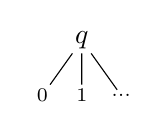
\begin{tikzpicture}[baseline=(root.base),level distance=7mm,inner ysep=0.5mm,sibling distance=5mm]
 \node (root) {$q$}
    child {node {$\scriptstyle 0$}}
    child {node {$\scriptstyle 1$}}
    child {node {$\scriptstyle \ldots$}}
;
\end{tikzpicture}$
\hspace{2cm}
$\sem{\nat \rightarrow \nat} = 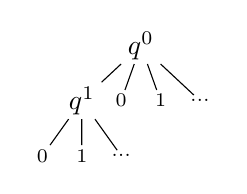
\begin{tikzpicture}[baseline=(root.base),level distance=7mm,inner ysep=0.5mm,sibling distance=5mm]
 \node (root) {$q^0$}
    child{
      node{$q^1$}
      child{node {$\scriptstyle 0$} }
      child{node {$\scriptstyle 1$} }
      child {node {$\scriptstyle \ldots$}}
    }
    child {node {$\scriptstyle 0$}}
    child {node {$\scriptstyle 1$}}
    child {node {$\scriptstyle \ldots$}}
;
\end{tikzpicture}$
\item \highlight{Play} = sequence of moves played alternatively by O and P with justification pointers.
\item \highlight{Strategy for P} = prefix-closed set of plays. $s  a  b$ in the strategy means that
P should respond $b$ when O plays $a$ in position $s$.
\item The \highlight{denotation} of a term $M$, written $\sem{M}$, is a strategy for P.
\item $\sem{ 7 : \nat} = \{ \epsilon, q, q\ 7 \}$\\
$\sem{ \pcfsucc : \nat \rightarrow \nat} = Pref( \{ q^0 q^1 n ( n+1)
\ | \ n \in \nat \} )$
\item Compositionality: $\sem{ \pcfsucc\  7} = \sem{ \pcfsucc } ; \sem{7}$
\end{itemize}
}

\def\highlightat#1#2{\temporal<#1>{#2}{\underline{#2}}{\textcolor{blue}{#2}}}

\section{Computation trees and traversals}
\frame{ \frametitle{Computation trees and traversals}
\highlight{\it Computation tree:} AST of the $\eta$-long normal form of a term.

Example: $M \equiv \lambda f z .
(\lambda g x . f x) (\lambda y. y) z$ of type $(o \typear o) \typear
o \typear o$. \vspace{0.5cm}
\begin{columns}
\column{6cm}
 \visible<2->{\highlight{\it Traversal:} justified
sequence of nodes representing the computation. }

\setbox0=\hbox{$\textcolor{blue}{
\pstr{\only<3->{\nd t= (q1){\lambda f z}}
        \only<4->{\nd \cdot (n2-q1) {@}}
        \only<5->{\nd \cdot (n3-n2){\lambda g x}}
        \only<6->{\nd \cdot (q3-q1,35){f}}
        \only<7->{\nd \cdot (q4-q3){\lambda}}
        \only<8->{\nd \cdot (n8-n3,35){x}}
        \only<9->{\nd \cdot (n9-n2,30){\lambda}}
        \only<10->{\nd \cdot (q2-q1,30){z}}
}}$}
\ht0 1cm\box0 % Make sure the height of box containing the traversal remains constant across the different generated slides

\vspace*{0.5cm}
\visible<11->{\highlight{\it Traversal reduction:} keep only
nodes hereditarily justified by the root.
$\color{red}{
\Pstr[0.7cm]{t \upharpoonright r = (q1){\lambda f z} \cdot (q3-q1,50){f}
\cdot (q4-q3,50){\lambda} \cdot (q2-q1){z} } }$
}

\vspace*{0.8cm}
\visible<12->{
\highlight{\it @-nodes removal:}
 $\Pstr[0.7cm]{ t - @ = (q1){\lambda f z}
 \cdot (n3-q1){ \lambda g x}
 \cdot (q3-q1,35){ f}
 \cdot (q4-q3){ \lambda}
 \cdot (n8-n3,30){ x}
 \cdot (n9-q1,30){ \lambda}
 \cdot (q2-q1,35){z}
} $}
\column{3.5cm}
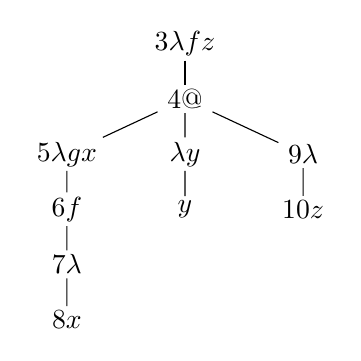
\begin{tikzpicture}[level distance=7mm,inner ysep=0.5mm]
 \node {\highlightat{3}{$\lambda f z$}}
    child {
        node {\highlightat{4}{@}}
        child {
            node {\highlightat{5}{$\lambda g x$}}
            child{
                node{\highlightat{6}{$f$}}
                child {
                    node{\highlightat{7}{$\lambda$}}
                    child {
                        node{\highlightat{8}{$x$}}
                    }
                }
            }
        }
        child {
            node {$\lambda y$}
            child{ node {$y$} }
        }
        child {
            node {$\highlightat{9}{\lambda}$}
            child{ node {\highlightat{10}{$z$}} }
            }
        };
\end{tikzpicture}
\end{columns}
}

%%%%%%%%%%%%%%%%%%%%%%%%%%%%%%%%%%%%%%%%%%%%%%%%%

\section{The Correspondence Theorem}
\frame{ \frametitle{The Correspondence Theorem}
\begin{block}{}
Let $M$ be a simply typed term of type $T$. There exists a partial function $\textcolor{DarkGreen}{\varphi}$
from the nodes of the \highlight{computation tree} to the
moves of the \highlight{arena} $\sem{T}$ such that
$$ \textcolor{DarkGreen}{\varphi}  : \travset(M)^{-@} \textcolor{DarkGreen}{\stackrel{\cong}{\longrightarrow}} \intersem{M} $$
$$ \textcolor{DarkGreen}{\varphi}  : \travset(M)^{\upharpoonright r}  \textcolor{DarkGreen}{\stackrel{\cong}{\longrightarrow}} \sem{M} \ .$$
\end{block}
where
\begin{itemize}
\item $\highlight{\travset(M)}$ = set of traversals of the computation tree of $M$
\item $\highlight{\travset(M)^{\upharpoonright r}} = \{ t \upharpoonright r \ | \  t \in {\travset(M)} \}$
\item $\highlight{\travset(M)^{-@}} = \{ t - @ \ | \  t \in {\travset(M)} \}$
\item $\highlight{\sem{M}}$ = game-semantic denotation of $M$
\item $\highlight{\intersem{M}}$ = revealed denotion ({\it i.e.}~internal moves are uncovered.)
\end{itemize}

}

%%%%%%%%%%%%%%%%%%%%%%%%%%%%%%%%%%%%%%%%%%%%%%%%%
\section{The Correspondence Theorem (example)}
\frame{\frametitle{The Correspondence Theorem (example)}
\begin{center}
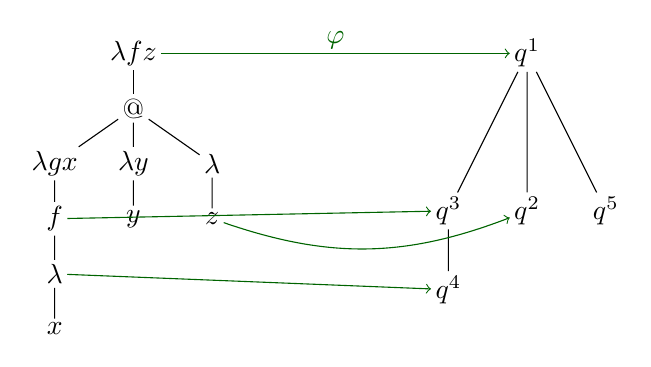
\begin{tikzpicture}[level distance=7mm,inner ysep=0.5mm,inner xsep=0.5mm,sibling distance=10mm]
%\color{blue}
\node (root) {$\lambda f z$}
    child{
      node{$@$}
          child{
            node {$\lambda g x$}
            child{
              node (f) {$f$}
              child{
                node (lmd) {$\lambda$}
                child{
                  node {$x$}
                }
              }
            }
          }
          child{
            node {$\lambda y$}
            child{
              node {$y$}
            }
          }
          child{
            node {$\lambda$}
            child{
              node (z) {$z$}
            }
          }
      }
;
%\color{red}
\draw +(5,0) node (q1) {$q^1$}
    [level distance=20mm]
      child{
        node (q3) {$q^3$}
        [level distance=10mm]
        child{ node (q4) {$q^4$} }
      }
      child{ node (q2) {$q^2$} }
      child{ node (q5) {$q^5$} }
;
\color{DarkGreen}
\draw[->] (root) -- node[above] {$\varphi$} (q1);
\draw[->] (f) -- (q3);
\draw[->] (lmd) -- (q4);
\draw[->] (z) to [bend right=20]  (q2);
\end{tikzpicture}
\end{center}
Take the traversal
%\textcolor{blue}
{\Pstr{t = (q1){\lambda f z} \cdot (n2){@}
\cdot (n3-n2){\lambda g x}
\cdot (q3-q1,35){f}
\cdot (q4-q3){\lambda}
\cdot (n8-n3){x}
\cdot (n9-n2,35){\lambda}
\cdot (q2-q1,35){z}}}. We have:
$
\textcolor{DarkGreen}{
\varphi (} %\textcolor{blue}
{t \upharpoonright r}
\textcolor{DarkGreen}{)} = \textcolor{DarkGreen}{\varphi (}
\textcolor{blue}{
\Pstr[70mm]{ (q1){\lambda f z}
            \cdot (q3-q1){f}
            \cdot (q4-q3){\lambda}
            \cdot (q2-q1){z} }
}
\textcolor{DarkGreen}{)} = %\textcolor{red}
{
\Pstr[70mm]{
    (q1){q}^1\
    (q3-q1){q}^3\
    (q4-q3){q}^4\
    (q2-q1){q}^2
}}
\in %\textcolor{red}
{\sem{M}}.
$
}

%%%%%%%%%%%%%%%%%%%%%%%%%%%%%%%%%%%%%%%%%%%%%%%%%

\section{The Correspondence Theorem (2)}
\frame{ \frametitle{The Correspondence Theorem (2)}
\begin{center}
\begin{tabular}{c|c}
Computation tree notion & Game-semantic equivalent \\ \hline \hline \\
computation tree & arena \\ \\
traversals & uncovered plays \\ \\
reduced traversal & plays \\ \\
paths in the computation tree & P-views of uncovered plays
\end{tabular}
\end{center}
}


%%%%%%%%%%%%%%%%%%%%%%%%%%%%%%%%%%%%%%%%%%%%%%%%%

\section{Game-semantic Characterisation of Safety}
\frame{ \frametitle{Game-semantic Characterisation of Safety}

\begin{itemize}
\item The computation tree of  a safe term is \highlight{incrementally-bound} :
each variable $x$ is bound by the first $\lambda$-node occurring in
\textcolor{red}{the path to the root} with order $> \ord{x}$.
\pause

\item Using the Correspondence Theorem, since paths in the computation tree correspond to P-views
of plays in game semantic, we can show:

\begin{block}{Proposition}
Safe terms are denoted by \highlight{P-incrementally justified strategies}: each P-move $m$ points to the
last O-move in \textcolor{red}{the P-view} with order $> \ord{m}$.
\end{block}
\end{itemize}
\pause

\begin{block}{Corollary}
Justification pointers attached to P-moves are redundant in the game-semantics of safe
terms.
\end{block}
}




%%%%%%%%%%%%%%%%%%%%%%%%%%%%%%%%%%%%%%%%%%%%%%%%%
\section{Conclusion and Future Works}
\frame{ \frametitle{Conclusion and Future Works}

\highlight{Conclusion:}

Safety is a syntactic constraint with interesting algorithmic and
game-semantic properties.

\highlight{Future works:}
\begin{itemize}
\item Find a categorical model of Safe PCF.
\item Complexity classes characterised with the Safe $\lambda$-calculus?
\item Safe Idealized Algol: is contextual equivalence decidable
for some finitary fragment (e.g.~Safe IA$_4$)?
\end{itemize}


\highlight{Related works:}
\begin{itemize}
\item Jolie G. de Miranda's thesis on unsafe grammars.
\item Ong introduced computation trees in LICS2006 to prove decidability of MSO theory on infinite trees
generated by higher-order grammars (whether safe or not).
%\item Stirling recently proved decidability of higher-order pattern matching with a game-semantic approach
%relying on equivalent notions of computation tree and traversal.
\end{itemize}
}


%%%%%%%%%%%%%%%%%%%%%%%%%%%%%%%%%%%%%%%%%%%%%%%%%
\section{Bibliography}

\end{document}
\endinput

\begin{frame} \frametitle<presentation>{Bibliography}

%  \begin{thebibliography}{10}
  \beamertemplatearticlebibitems
    \bibitem{abramsky:game-semantics-tutorial}
    Samson Abramsky and Guy McCusker.
    \newblock Game semantics, Lecture notes.
    \newblock In {\em Proceedings of the 1997 Marktoberdorf Summer School}. Springer-Verlag, 1998.

    \bibitem{safety-mirlong2004}
    Klaus Aehlig, Jolie~G. de~Miranda, and C.-H.~Luke Ong.
    \newblock Safety is not a restriction at level 2 for string languages.
    \newblock Technical report. University of Oxford, 2004.

    \bibitem{OngLics2006}
    C.-H.~Luke Ong.
    \newblock On model-checking trees generated by higher-order recursion schemes.
    \newblock In {\em Proceedings of LICS.} Computer Society Press, 2006.

%    \bibitem{DBLP:conf/icalp/Stirling06}
%    Colin Stirling
%    \newblock A Game-Theoretic Approach to Deciding Higher-Order Matching.
%    \newblock In {\em Proceedings of ICALP.} Springer, 2006.

%  \end{thebibliography}
\end{frame}

\end{document}


\pstrSetArrowColor{black}

\title{\texorpdfstring{The Safe $\lambda$-Calculus}{The Safe Lambda-Calculus}}

\author[W. Blum, C.-H. L. Ong]{\texorpdfstring{\\ William Blum\\ \ \\
 Joint work with C.-H. Luke Ong}{William Blum}}


\institute[University Of Oxford]{Oxford University Computing Laboratory}

\date{\small \color{red}{Lunch-time meeting, 14 May 2007}}


\begin{document}

\section{Title page}
  \frame{\titlepage}


%\section<presentation>*{Outline}
%\begin{frame}
%  \frametitle{Outline}
%  \tableofcontents[part=1]
%\end{frame}
%\AtBeginSection[] {
%   \begin{frame}<beamer>
%     \frametitle{Outline}
%     \tableofcontents[currentpart,currentsection]
%   \end{frame}
% }
%
%\part<presentation>{Main Talk}

%%%%%%%%%%%%%%%%%%%%%%%%%%%%%%%%%%%%%%%%%%%%%%%%%

\section{Overview}
\frame{\frametitle{Overview}

\begin{itemize}
\item \highlight{Safety} is originally a syntactic restriction for higher-order grammars
with nice automata-theoretic characterization.
\item In the context of the $\lambda$-calculus it gives rise to the \highlight{Safe $\lambda$-calculus}.
\item The loss of expressivity can be characterized in terms of representable numeric functions.
\item The calculus has a ``succinct'' game-semantic model ({\it i.e.}~in terms of pointers needed).
\end{itemize}
}


%%%%%%%%%%%%%%%%%%%%%%%%%%%%%%%%%%%%%%%%%%%%%%%%%

\section{Outline for this talk}
\frame{
\frametitle{Outline for this talk}
\begin{enumerate}
\item The safety restriction
%\item The simply typed $\lambda$-calculus
\item The safe $\lambda$-calculus
\item Numeric function representable
\item Game-semantic characterisation
\end{enumerate}
}


\part{The Safety Restriction}


\section{Higher-order grammars}
\frame{\frametitle{Higher-order grammars}
\emph{Notation for types:} $A_1 \rightarrow (A_2 \rightarrow (\ldots (A_n \rightarrow o)) \ldots )$
is written $(A_1,A_2,\ldots, A_n,o)$.

\begin{itemize}

\item \highlight{Higher-grammars} formally given by a tuple
$\langle \Sigma, \mathcal{N}, \mathcal{R}, \mathcal{S} \rangle$
(terminals, non-terminals, rewritting rules, starting symbol)

\item They are used as generators for word language, trees or graphs.


\item Example of a tree generating order-2 grammar:
\begin{columns}
      \column{.3\textwidth}
$\begin{array}{rll}
  S & \rightarrow & H \, a\\
  H \, z^o & \rightarrow & F \, (g \,
  z)\\
  F \, \phi^{(o, o)} & \rightarrow & \phi \, (\phi \, (F \, h))\\
\end{array}$
      \column{.3\textwidth}
\begin{tikzpicture}[baseline=(root.base),level distance=5mm,inner ysep=0.5mm,sibling distance=10mm]
 \node (root) {$g$}
    child {node {$a$}}
    child {node {$g$}
        child { node{$a$} }
        child { node{$h$}
                child { node{$h$}
                        child { node{$\vdots$} }
                }
        }
    } ;
\end{tikzpicture}
\end{columns}
The non-terminals are $S, H, F$ of type $o$, $(o,o)$ and $((o,o),o)$ respectively. The terminals are $a:o$ and $g,h:(o,o)$.
\end{itemize}
}

%%%%%%%%%%%%%%%%%%%%%%%%%%%%%%%%%%%%%%%%%%%%%%%%%
\section{The Safety Restriction}
\frame{\frametitle{The Safety Restriction}
\begin{itemize}
\item First appeared under the name ``restriction of derived types'' in ``IO and OI Hierarchies'' by W. Damm, TCS 1982
\item It is a \highlight{syntactic restriction} for higher-order grammars that constrains the occurrences
of the variables in the grammar equations according to their orders.
\pause

\item $(A_1, \cdots, A_n, o)$ is \highlight{homogeneous} if
$A_1$, \ldots, $A_n$ are and $\ord{A_1} \geq \ord{A_2}\geq \cdots \geq \ord{A_n}$.
\end{itemize}

\begin{definition}[Knapik, Niwi\'nski and Urzyczyn (2001-2002)]
\noindent All types are assumed to be \emph{homogeneous}.

  An order $k > 0$ term is \emph{unsafe} if it contains an
  occurrence of a parameter of order strictly less than $k$.
  An unsafe subterm $t$ of $t'$ occurs in \emph{safe position}
  if it is in operator position ($t' = \cdots (ts) \cdots$).
  A grammar is \highlight{safe} if at the right-hand side of any production
  all unsafe subterms occur in safe position.
\end{definition}
}

\section{Some Results On Safety}
\frame{\frametitle{Some Results On Safety}
\begin{description}
\item [Damm82] For generating word languages, order-$n$ safe grammars are
equivalent to order-$n$ pushdown automata.

\item [KNU02] Generalization of the previous result to
\emph{tree generating} safe grammars/PDAs.

\item [KNU02] The Monadic Second Order (MSO) model checking problem for trees generated by
    \highlight{safe} higher-order grammars of any order is decidable.

\item graphs Caucal MSO theory decidable. Hagues et al.: undecidable for unsafe grammars but
$\mu$-calculus is $n$-EXPTIME complete.
\end{description}


\note{
\begin{itemize}
\item nPDA = finite state machines + order n stack
\item For words: 1PDA recognizes context-free language.
        and 0PDA = recognizes regular language.
\item MSO is very expressive: more than the modal mu-calculus (into which LTL CTL CTL* can be embedded.
But over trees, MSO and modal mu-calculus are equi-expressive.)
\end{itemize}
}
}



%%%%%%%%%%%%%%%%%%%%%%%%%%%%%%%%%%%%%%%%%%%%%%%%%
\section{Simply Typed \texorpdfstring{$\lambda$}{Lambda}-Calculus}
\frame{\frametitle{Simply Typed $\lambda$-Calculus}
\begin{itemize}
\item \highlight{Simple types} $A := o\ |\ A \rightarrow A$.
%We write $(A_1,\ldots, A_n)$ for $A_1\rightarrow \ldots \rightarrow A_n$.
\pause
\item The \highlight{order} of a type is given by $\textsf{order}(o) = 0$,
$\textsf{order}(A \rightarrow B) = \max(\textsf{order}(A) + 1, \textsf{order}(B))$.
\pause
\item Jugdements of the form $ \Gamma \vdash M : T $ where $\Gamma$ is the context, $M$ is the term and $T$ is the type:
$$ \rulename{var} \   \rulef{}{x : A\vdash x : A}
\qquad  \rulename{wk} \   \rulef{\Gamma \vdash M : A}{\Delta \vdash M : A} \ \Gamma \subset \Delta$$
$$ \rulename{app} \  \rulef{\Gamma \vdash M : A \rightarrow B \quad \Gamma \vdash N : A }
                           {\Gamma  \vdash M N : B}
\quad \rulename{abs} \   \rulef{\Gamma, x : A \vdash M : B}
                                {\Gamma  \vdash \lambda x^A. M : A \rightarrow B}$$
\pause
\item Example: $f:o\rightarrow o\rightarrow o, x:o \vdash (\lambda \varphi^{o \rightarrow o} x^o . \varphi\ x) (f\ x)$
\pause
\item A single rule: \highlight{$\beta$-reduction}. e.g. $(\lambda x. M) N \betared M [N/x]$
\end{itemize}
}




%%%%%%%%%%%%%%%%%%%%%%%%%%%%%%%%%%%%%%%%%%%%%%%%%
\section{The Safe \texorpdfstring{$\lambda$}{Lambda}-Calculus}
\begin{frame} \frametitle{The Safe $\lambda$-Calculus}

In an unpublished technical report (2004),
Aehlig, de~Miranda and Ong  proposed
a notion of safety for the $\lambda$-calculus.

\begin{block}{The formation rules}
$$ \rulename{var} \   \rulef{}{x : A\vdash_s x : A}
\qquad  \rulename{wk} \   \rulef{\Gamma \vdash_s M : A}{\Delta \vdash_s
M : A} \ \Gamma \subset \Delta$$
$$ \rulename{app} \  \rulef{\Gamma \vdash M : (A_1,\ldots,A_l,B)
                                        \quad \Gamma \vdash_s N_1 : A_1
                                        \quad \ldots \quad \Gamma \vdash_s N_l : A_l  }
                                   {\Gamma  \vdash_s M N_1 \ldots N_l : B}$$
\hfill with the side-condition $\textcolor{red}{\forall y \in \Gamma
: \ord{y} \geq \ord{B}}$
$$ \rulename{abs} \   \rulef{\Gamma, x_1:A_1 \ldots x_n : A_n \vdash_s M : B}
                                   {\Gamma  \vdash_s \lambda x_1:A_1 \ldots x_n : A_n . M : A_1 \rightarrow \ldots \rightarrow A_n \rightarrow B}$$
\hfill with the side-condition $\textcolor{red}{\forall y \in \Gamma
: \ord{y} \geq \ord{A_1 \rightarrow \ldots \rightarrow A_n
\rightarrow B}}$
\end{block}

\begin{lemma}
  If $\Gamma \vdash_s M : A$ then every free variable in $M$ has order at least $\ord{A}$.
\end{lemma}

\end{frame}

%%%%%%%%%%%%%%%%%%%%%%%%%%%%%%%%%%%%%%%%%%%%%%%%%

\section{Variable Capture}
\frame{\frametitle{Variable Capture} \highlight{The usual
``problem'' in $\lambda$-calculus}: avoid \alert{variable capture}
when performing substitution: $ (\lambda x . (\lambda y . x)) y
\betared (\lambda \underline{y} . x) [\underline{y}/x] \neq \lambda
y . y$\pause
\begin{enumerate}
\item \highlight{Standard solution}: Barendregt's convention. Variables are renamed so that free variables and bound variables have different names.
Eg. $(\lambda x . (\lambda y . x)) y$ becomes $(\lambda x . (\lambda
z . x)) y$ which reduces to $(\lambda z . x) [y/x] = \lambda z . y$
\pause

\alert{Drawback:} requires to have access to an unbounded supply of names to perform
a given sequence of $\beta$-reductions.
\note{Drawback 1, eg. $(\lambda x_1 \ldots x_n . (\lambda y_1 \ldots y_n . x_1 \ldots x_n)) y_1 \ldots y_n$}
\pause

\item \highlight{Another solution}: use the $\lambda$-calculus \`a la de Brujin where variable binding is specified by an index instead of a name.
Variable renaming then becomes unnecessary.
\pause

\alert{Drawback:} the conversion to nameless de Brujin $\lambda$-terms requires an unbounded supply of indices.
\pause
\end{enumerate}

\alert{The Safety restriction avoids the need for variable renaming:}
\begin{block}{Property}
In the Safe $\lambda$-calculus there is no need to rename variables when
performing substitution.
\end{block} 

}

%%%%%%%%%%%%%%%%%%%%%%%%%%%%%%%%%%%%%%%%%%%%%%%%%
\section{Examples}
\frame{\frametitle{Examples}
\begin{enumerate}
\item
Contracting the $\beta$-redex in the following term
$$f:o\rightarrow o\rightarrow o, x:o \vdash (\lambda \varphi^{o \rightarrow o} x^o . \varphi\ x) (\temporal<2>{f\ x}{\underline{f\ \alert{x}}}{\underline{f\ \alert{x}}})$$
leads to variable capture:
$$(\lambda \varphi x . \varphi\ x) (f\ x) \not\betared (\lambda \alert{x} . (f\ \alert{x}) x).$$
\pause
Hence the term is \alert{unsafe}.

Indeed, $\ord{x} = 0 \leq 1 = \ord{f\ x}$.
\pause

\item The term $(\lambda \varphi^{o \rightarrow o} x^o . \varphi\ x) (\lambda y^o . y )$ is safe.

\item Safety does not capture ``variable-capture uselessness'': the unsafe term
$\lambda y^o z^o. (\lambda x^o .y) z$ can be contracted using capture-permitting substitution.

\item Kierstead terms: $M_1 = \lambda f^{((o,o),o)} . f (\lambda x^o . f (\lambda y^o . y
))$ is safe. However $M_2 = \lambda f^{((o,o),o)} . f (\lambda x^o . f (\underline{\lambda y^o .x}))$
is unsafe because in the ground free variable $x$ occurs in the underlined order-1 subterm
which is at operand position.
\end{enumerate}
}

%%%%%%%%%%%%%%%%%%%%%%%%%%%%%%%%%%%%%%%%%%%%%%%%%
\section{Transformations preserving safety}
\frame{\frametitle{Transformations preserving safety}
\begin{itemize}
  \item Substitution preserves safety
  \item $\beta$-reduction does not preserve safety:
Take  $w,x,y,z : o$ and $f : (o,o,o)$.
The safe term $(\lambda x y . f x y) z w$
$\beta$-reduces to the unsafe term $(\underline{\lambda y . f z y}) w$
which in turns reduces to the safe term $f z w$.

  \item Safe $\beta$-reduction:

  \item Safe $\beta$-reduction preserves safety,
  \item $\eta$-reduction preserves safety,
  \item $\eta$-expansion \alert{does not} preserve safety,
  \item $\eta$-long normal expansion preserves safety.
\end{itemize}

}


%%%%%%%%%%%%%%%%%%%%%%%%%%%%%%%%%%%%%%%%%%%%%%%%%
\section{Numerical functions}
\frame{ \frametitle{Numerical functions}

Church Encoding: for $n\in\nat$, $\overline{n} = \lambda s z. s^n z$
of type $I = (o\rightarrow o)\rightarrow o\rightarrow o$.

\begin{theorem}[Schwichtenberg 1976]
The numeric functions representable by simply-typed terms of type $I\rightarrow \ldots \rightarrow I$ are
exactly the multivariate polynomials extended with the conditional function:
$$ cond(t,x,y) =
\left\{ \begin{array}{ll} x, & \mbox{if $t=0$} \\
y, & \mbox{if $t = n+1$}\ .
\end{array} \right.
$$
\end{theorem}
$cond$ is represented by the term $C = \lambda F G H \alpha x . H (
\temporal<2>{\lambda y . G \alpha x}
{\underline{\lambda y . G \alpha x}}{\underline{\lambda y . G \alpha x}}
 ) (F \alpha x)$.
\pause
\begin{theorem}
Functions representable  by safe $\lambda$-expressions of type $I\rightarrow \ldots \rightarrow I$  are
exactly the multivariate polynomials.
\end{theorem}
So $cond$ is not representable in the Safe $\lambda$-calculus and $C$ is unsafe.
}

%%%%%%%%%%%%%%%%%%%%%%%%%%%%%%%%%%%%%%%%%%%%%%%%%

%%%%\section{Game Semantics}
%%%%\frame{ \frametitle{Game Semantics}
%%%%Let $\vdash M:T$ be a pure simply typed term.
%%%%
%%%%\begin{itemize}
%%%%\item \highlight{Game-semantics} provides a model of $\lambda$-calculus.
%%%%$M$ is denoted by a strategy $\sem{M}$ on a 2-player game induced by $T$.
%%%%\item A \highlight{strategy} is represented by a set of sequences of moves together with \highlight{links}: each move points
%%%%to a preceding move.
%%%%\pause
%%%%\item \textcolor{DarkGreen}{Computation tree} = canonical tree representation of a term.
%%%%\item \textcolor{DarkGreen}{Traversals $\travset(M)$ } = sequences of nodes with links respecting some formation rules.
%%%%\end{itemize}
%%%%\pause
%%%%
%%%%\begin{block}{The Correspondence Theorem}
%%%%The game semantics of a term can be represented on the computation
%%%%tree:
%%%%$$ \textcolor{DarkGreen}{\travset(M)} \cong \textcolor{blue}{\intersem{M}} $$
%%%%$$ \textcolor{DarkGreen}{Reduction(\travset(M))} \cong \textcolor{blue}{\sem{M}}$$
%%%%where $\textcolor{blue}{\intersem{M}}$ is the revealed game-semantic denotion (i.e. internal moves are uncovered).
%%%%\end{block}
%%%%}


%%%%%%%%%%%%%%%%%%%%%%%%%%%%%%%%%%%%%%%%%%%%%%%%%

\part{Game semantics}

\section{Game semantics}
\frame{\frametitle{Game semantics}
 Model of programming languages based on games (Abramsky et al.; Hyland and Ong; Nickau)
\begin{itemize}
\item 2 players: \highlight{O}pponnent (system) and \highlight{P}roponent (program)
\item The term type induces an \highlight{arena} defining the possible moves
$\sem{\nat} = 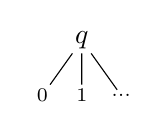
\begin{tikzpicture}[baseline=(root.base),level distance=7mm,inner ysep=0.5mm,sibling distance=5mm]
 \node (root) {$q$}
    child {node {$\scriptstyle 0$}}
    child {node {$\scriptstyle 1$}}
    child {node {$\scriptstyle \ldots$}}
;
\end{tikzpicture}$
\hspace{2cm}
$\sem{\nat \rightarrow \nat} = 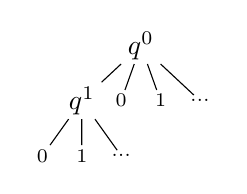
\begin{tikzpicture}[baseline=(root.base),level distance=7mm,inner ysep=0.5mm,sibling distance=5mm]
 \node (root) {$q^0$}
    child{
      node{$q^1$}
      child{node {$\scriptstyle 0$} }
      child{node {$\scriptstyle 1$} }
      child {node {$\scriptstyle \ldots$}}
    }
    child {node {$\scriptstyle 0$}}
    child {node {$\scriptstyle 1$}}
    child {node {$\scriptstyle \ldots$}}
;
\end{tikzpicture}$
\item \highlight{Play} = sequence of moves played alternatively by O and P with justification pointers.
\item \highlight{Strategy for P} = prefix-closed set of plays. $s  a  b$ in the strategy means that
P should respond $b$ when O plays $a$ in position $s$.
\item The \highlight{denotation} of a term $M$, written $\sem{M}$, is a strategy for P.
\item $\sem{ 7 : \nat} = \{ \epsilon, q, q\ 7 \}$\\
$\sem{ \pcfsucc : \nat \rightarrow \nat} = Pref( \{ q^0 q^1 n ( n+1)
\ | \ n \in \nat \} )$
\item Compositionality: $\sem{ \pcfsucc\  7} = \sem{ \pcfsucc } ; \sem{7}$
\end{itemize}
}

\def\highlightat#1#2{\temporal<#1>{#2}{\underline{#2}}{\textcolor{blue}{#2}}}

\section{Computation trees and traversals}
\frame{ \frametitle{Computation trees and traversals}
\highlight{\it Computation tree:} AST of the $\eta$-long normal form of a term.

Example: $M \equiv \lambda f z .
(\lambda g x . f x) (\lambda y. y) z$ of type $(o \typear o) \typear
o \typear o$. \vspace{0.5cm}
\begin{columns}
\column{6cm}
 \visible<2->{\highlight{\it Traversal:} justified
sequence of nodes representing the computation. }

\setbox0=\hbox{$\textcolor{blue}{
\pstr{\only<3->{\nd t= (q1){\lambda f z}}
        \only<4->{\nd \cdot (n2-q1) {@}}
        \only<5->{\nd \cdot (n3-n2){\lambda g x}}
        \only<6->{\nd \cdot (q3-q1,35){f}}
        \only<7->{\nd \cdot (q4-q3){\lambda}}
        \only<8->{\nd \cdot (n8-n3,35){x}}
        \only<9->{\nd \cdot (n9-n2,30){\lambda}}
        \only<10->{\nd \cdot (q2-q1,30){z}}
}}$}
\ht0 1cm\box0 % Make sure the height of box containing the traversal remains constant across the different generated slides

\vspace*{0.5cm}
\visible<11->{\highlight{\it Traversal reduction:} keep only
nodes hereditarily justified by the root.
$\color{red}{
\Pstr[0.7cm]{t \upharpoonright r = (q1){\lambda f z} \cdot (q3-q1,50){f}
\cdot (q4-q3,50){\lambda} \cdot (q2-q1){z} } }$
}

\vspace*{0.8cm}
\visible<12->{
\highlight{\it @-nodes removal:}
 $\Pstr[0.7cm]{ t - @ = (q1){\lambda f z}
 \cdot (n3-q1){ \lambda g x}
 \cdot (q3-q1,35){ f}
 \cdot (q4-q3){ \lambda}
 \cdot (n8-n3,30){ x}
 \cdot (n9-q1,30){ \lambda}
 \cdot (q2-q1,35){z}
} $}
\column{3.5cm}
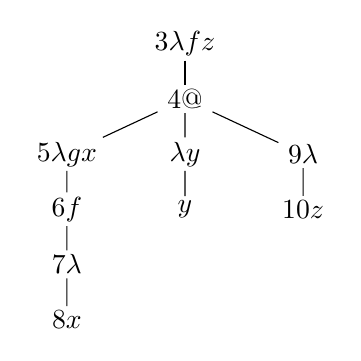
\begin{tikzpicture}[level distance=7mm,inner ysep=0.5mm]
 \node {\highlightat{3}{$\lambda f z$}}
    child {
        node {\highlightat{4}{@}}
        child {
            node {\highlightat{5}{$\lambda g x$}}
            child{
                node{\highlightat{6}{$f$}}
                child {
                    node{\highlightat{7}{$\lambda$}}
                    child {
                        node{\highlightat{8}{$x$}}
                    }
                }
            }
        }
        child {
            node {$\lambda y$}
            child{ node {$y$} }
        }
        child {
            node {$\highlightat{9}{\lambda}$}
            child{ node {\highlightat{10}{$z$}} }
            }
        };
\end{tikzpicture}
\end{columns}
}

%%%%%%%%%%%%%%%%%%%%%%%%%%%%%%%%%%%%%%%%%%%%%%%%%

\section{The Correspondence Theorem}
\frame{ \frametitle{The Correspondence Theorem}
\begin{block}{}
Let $M$ be a simply typed term of type $T$. There exists a partial function $\textcolor{DarkGreen}{\varphi}$
from the nodes of the \highlight{computation tree} to the
moves of the \highlight{arena} $\sem{T}$ such that
$$ \textcolor{DarkGreen}{\varphi}  : \travset(M)^{-@} \textcolor{DarkGreen}{\stackrel{\cong}{\longrightarrow}} \intersem{M} $$
$$ \textcolor{DarkGreen}{\varphi}  : \travset(M)^{\upharpoonright r}  \textcolor{DarkGreen}{\stackrel{\cong}{\longrightarrow}} \sem{M} \ .$$
\end{block}
where
\begin{itemize}
\item $\highlight{\travset(M)}$ = set of traversals of the computation tree of $M$
\item $\highlight{\travset(M)^{\upharpoonright r}} = \{ t \upharpoonright r \ | \  t \in {\travset(M)} \}$
\item $\highlight{\travset(M)^{-@}} = \{ t - @ \ | \  t \in {\travset(M)} \}$
\item $\highlight{\sem{M}}$ = game-semantic denotation of $M$
\item $\highlight{\intersem{M}}$ = revealed denotion ({\it i.e.}~internal moves are uncovered.)
\end{itemize}

}

%%%%%%%%%%%%%%%%%%%%%%%%%%%%%%%%%%%%%%%%%%%%%%%%%
\section{The Correspondence Theorem (example)}
\frame{\frametitle{The Correspondence Theorem (example)}
\begin{center}
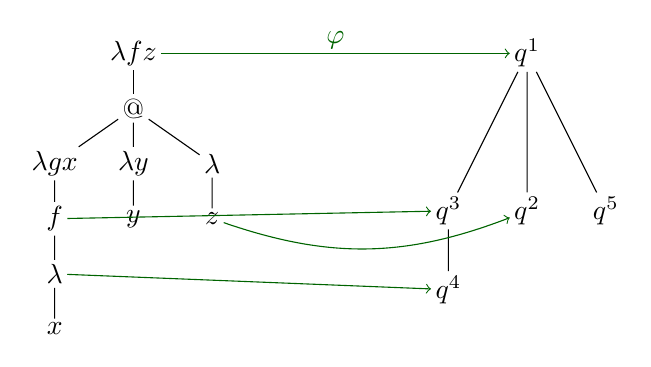
\begin{tikzpicture}[level distance=7mm,inner ysep=0.5mm,inner xsep=0.5mm,sibling distance=10mm]
%\color{blue}
\node (root) {$\lambda f z$}
    child{
      node{$@$}
          child{
            node {$\lambda g x$}
            child{
              node (f) {$f$}
              child{
                node (lmd) {$\lambda$}
                child{
                  node {$x$}
                }
              }
            }
          }
          child{
            node {$\lambda y$}
            child{
              node {$y$}
            }
          }
          child{
            node {$\lambda$}
            child{
              node (z) {$z$}
            }
          }
      }
;
%\color{red}
\draw +(5,0) node (q1) {$q^1$}
    [level distance=20mm]
      child{
        node (q3) {$q^3$}
        [level distance=10mm]
        child{ node (q4) {$q^4$} }
      }
      child{ node (q2) {$q^2$} }
      child{ node (q5) {$q^5$} }
;
\color{DarkGreen}
\draw[->] (root) -- node[above] {$\varphi$} (q1);
\draw[->] (f) -- (q3);
\draw[->] (lmd) -- (q4);
\draw[->] (z) to [bend right=20]  (q2);
\end{tikzpicture}
\end{center}
Take the traversal
%\textcolor{blue}
{\Pstr{t = (q1){\lambda f z} \cdot (n2){@}
\cdot (n3-n2){\lambda g x}
\cdot (q3-q1,35){f}
\cdot (q4-q3){\lambda}
\cdot (n8-n3){x}
\cdot (n9-n2,35){\lambda}
\cdot (q2-q1,35){z}}}. We have:
$
\textcolor{DarkGreen}{
\varphi (} %\textcolor{blue}
{t \upharpoonright r}
\textcolor{DarkGreen}{)} = \textcolor{DarkGreen}{\varphi (}
\textcolor{blue}{
\Pstr[70mm]{ (q1){\lambda f z}
            \cdot (q3-q1){f}
            \cdot (q4-q3){\lambda}
            \cdot (q2-q1){z} }
}
\textcolor{DarkGreen}{)} = %\textcolor{red}
{
\Pstr[70mm]{
    (q1){q}^1\
    (q3-q1){q}^3\
    (q4-q3){q}^4\
    (q2-q1){q}^2
}}
\in %\textcolor{red}
{\sem{M}}.
$
}

%%%%%%%%%%%%%%%%%%%%%%%%%%%%%%%%%%%%%%%%%%%%%%%%%

\section{The Correspondence Theorem (2)}
\frame{ \frametitle{The Correspondence Theorem (2)}
\begin{center}
\begin{tabular}{c|c}
Computation tree notion & Game-semantic equivalent \\ \hline \hline \\
computation tree & arena \\ \\
traversals & uncovered plays \\ \\
reduced traversal & plays \\ \\
paths in the computation tree & P-views of uncovered plays
\end{tabular}
\end{center}
}


%%%%%%%%%%%%%%%%%%%%%%%%%%%%%%%%%%%%%%%%%%%%%%%%%

\section{Game-semantic Characterisation of Safety}
\frame{ \frametitle{Game-semantic Characterisation of Safety}

\begin{itemize}
\item The computation tree of  a safe term is \highlight{incrementally-bound} :
each variable $x$ is bound by the first $\lambda$-node occurring in
\textcolor{red}{the path to the root} with order $> \ord{x}$.
\pause

\item Using the Correspondence Theorem, since paths in the computation tree correspond to P-views
of plays in game semantic, we can show:

\begin{block}{Proposition}
Safe terms are denoted by \highlight{P-incrementally justified strategies}: each P-move $m$ points to the
last O-move in \textcolor{red}{the P-view} with order $> \ord{m}$.
\end{block}
\end{itemize}
\pause

\begin{block}{Corollary}
Justification pointers attached to P-moves are redundant in the game-semantics of safe
terms.
\end{block}
}




%%%%%%%%%%%%%%%%%%%%%%%%%%%%%%%%%%%%%%%%%%%%%%%%%
\section{Conclusion and Future Works}
\frame{ \frametitle{Conclusion and Future Works}

\highlight{Conclusion:}

Safety is a syntactic constraint with interesting algorithmic and
game-semantic properties.

\highlight{Future works:}
\begin{itemize}
\item Find a categorical model of Safe PCF.
\item Complexity classes characterised with the Safe $\lambda$-calculus?
\item Safe Idealized Algol: is contextual equivalence decidable
for some finitary fragment (e.g.~Safe IA$_4$)?
\end{itemize}


\highlight{Related works:}
\begin{itemize}
\item Jolie G. de Miranda's thesis on unsafe grammars.
\item Ong introduced computation trees in LICS2006 to prove decidability of MSO theory on infinite trees
generated by higher-order grammars (whether safe or not).
%\item Stirling recently proved decidability of higher-order pattern matching with a game-semantic approach
%relying on equivalent notions of computation tree and traversal.
\end{itemize}
}


%%%%%%%%%%%%%%%%%%%%%%%%%%%%%%%%%%%%%%%%%%%%%%%%%
\section{Bibliography}

\end{document}
\endinput

\begin{frame} \frametitle<presentation>{Bibliography}

%  \begin{thebibliography}{10}
  \beamertemplatearticlebibitems
    \bibitem{abramsky:game-semantics-tutorial}
    Samson Abramsky and Guy McCusker.
    \newblock Game semantics, Lecture notes.
    \newblock In {\em Proceedings of the 1997 Marktoberdorf Summer School}. Springer-Verlag, 1998.

    \bibitem{safety-mirlong2004}
    Klaus Aehlig, Jolie~G. de~Miranda, and C.-H.~Luke Ong.
    \newblock Safety is not a restriction at level 2 for string languages.
    \newblock Technical report. University of Oxford, 2004.

    \bibitem{OngLics2006}
    C.-H.~Luke Ong.
    \newblock On model-checking trees generated by higher-order recursion schemes.
    \newblock In {\em Proceedings of LICS.} Computer Society Press, 2006.

%    \bibitem{DBLP:conf/icalp/Stirling06}
%    Colin Stirling
%    \newblock A Game-Theoretic Approach to Deciding Higher-Order Matching.
%    \newblock In {\em Proceedings of ICALP.} Springer, 2006.

%  \end{thebibliography}
\end{frame}

\end{document}


\pstrSetArrowColor{black}

\title{\texorpdfstring{The Safe $\lambda$-Calculus}{The Safe Lambda-Calculus}}

\author[W. Blum, C.-H. L. Ong]{\texorpdfstring{\\ William Blum\\ \ \\
 Joint work with C.-H. Luke Ong}{William Blum}}


\institute[University Of Oxford]{Oxford University Computing Laboratory}

\date{\small \color{red}{Lunch-time meeting, 14 May 2007}}


\begin{document}

\section{Title page}
  \frame{\titlepage}


%\section<presentation>*{Outline}
%\begin{frame}
%  \frametitle{Outline}
%  \tableofcontents[part=1]
%\end{frame}
%\AtBeginSection[] {
%   \begin{frame}<beamer>
%     \frametitle{Outline}
%     \tableofcontents[currentpart,currentsection]
%   \end{frame}
% }
%
%\part<presentation>{Main Talk}

%%%%%%%%%%%%%%%%%%%%%%%%%%%%%%%%%%%%%%%%%%%%%%%%%

\section{Overview}
\frame{\frametitle{Overview}

\begin{itemize}
\item \highlight{Safety} is originally a syntactic restriction for higher-order grammars
with nice automata-theoretic characterization.
\item In the context of the $\lambda$-calculus it gives rise to the \highlight{Safe $\lambda$-calculus}.
\item The loss of expressivity can be characterized in terms of representable numeric functions.
\item The calculus has a ``succinct'' game-semantic model ({\it i.e.}~in terms of pointers needed).
\end{itemize}
}


%%%%%%%%%%%%%%%%%%%%%%%%%%%%%%%%%%%%%%%%%%%%%%%%%

\section{Outline for this talk}
\frame{
\frametitle{Outline for this talk}
\begin{enumerate}
\item The safety restriction
%\item The simply typed $\lambda$-calculus
\item The safe $\lambda$-calculus
\item Numeric function representable
\item Game-semantic characterisation
\end{enumerate}
}


\part{The Safety Restriction}


\section{Higher-order grammars}
\frame{\frametitle{Higher-order grammars}
\emph{Notation for types:} $A_1 \rightarrow (A_2 \rightarrow (\ldots (A_n \rightarrow o)) \ldots )$
is written $(A_1,A_2,\ldots, A_n,o)$.

\begin{itemize}

\item \highlight{Higher-grammars} formally given by a tuple
$\langle \Sigma, \mathcal{N}, \mathcal{R}, \mathcal{S} \rangle$
(terminals, non-terminals, rewritting rules, starting symbol)

\item They are used as generators for word language, trees or graphs.


\item Example of a tree generating order-2 grammar:
\begin{columns}
      \column{.3\textwidth}
$\begin{array}{rll}
  S & \rightarrow & H \, a\\
  H \, z^o & \rightarrow & F \, (g \,
  z)\\
  F \, \phi^{(o, o)} & \rightarrow & \phi \, (\phi \, (F \, h))\\
\end{array}$
      \column{.3\textwidth}
\begin{tikzpicture}[baseline=(root.base),level distance=5mm,inner ysep=0.5mm,sibling distance=10mm]
 \node (root) {$g$}
    child {node {$a$}}
    child {node {$g$}
        child { node{$a$} }
        child { node{$h$}
                child { node{$h$}
                        child { node{$\vdots$} }
                }
        }
    } ;
\end{tikzpicture}
\end{columns}
The non-terminals are $S, H, F$ of type $o$, $(o,o)$ and $((o,o),o)$ respectively. The terminals are $a:o$ and $g,h:(o,o)$.
\end{itemize}
}

%%%%%%%%%%%%%%%%%%%%%%%%%%%%%%%%%%%%%%%%%%%%%%%%%
\section{The Safety Restriction}
\frame{\frametitle{The Safety Restriction}
\begin{itemize}
\item First appeared under the name ``restriction of derived types'' in ``IO and OI Hierarchies'' by W. Damm, TCS 1982
\item It is a \highlight{syntactic restriction} for higher-order grammars that constrains the occurrences
of the variables in the grammar equations according to their orders.
\pause

\item $(A_1, \cdots, A_n, o)$ is \highlight{homogeneous} if
$A_1$, \ldots, $A_n$ are and $\ord{A_1} \geq \ord{A_2}\geq \cdots \geq \ord{A_n}$.
\end{itemize}

\begin{definition}[Knapik, Niwi\'nski and Urzyczyn (2001-2002)]
\noindent All types are assumed to be \emph{homogeneous}.

  An order $k > 0$ term is \emph{unsafe} if it contains an
  occurrence of a parameter of order strictly less than $k$.
  An unsafe subterm $t$ of $t'$ occurs in \emph{safe position}
  if it is in operator position ($t' = \cdots (ts) \cdots$).
  A grammar is \highlight{safe} if at the right-hand side of any production
  all unsafe subterms occur in safe position.
\end{definition}
}

\section{Some Results On Safety}
\frame{\frametitle{Some Results On Safety}
\begin{description}
\item [Damm82] For generating word languages, order-$n$ safe grammars are
equivalent to order-$n$ pushdown automata.

\item [KNU02] Generalization of the previous result to
\emph{tree generating} safe grammars/PDAs.

\item [KNU02] The Monadic Second Order (MSO) model checking problem for trees generated by
    \highlight{safe} higher-order grammars of any order is decidable.

\item graphs Caucal MSO theory decidable. Hagues et al.: undecidable for unsafe grammars but
$\mu$-calculus is $n$-EXPTIME complete.
\end{description}


\note{
\begin{itemize}
\item nPDA = finite state machines + order n stack
\item For words: 1PDA recognizes context-free language.
        and 0PDA = recognizes regular language.
\item MSO is very expressive: more than the modal mu-calculus (into which LTL CTL CTL* can be embedded.
But over trees, MSO and modal mu-calculus are equi-expressive.)
\end{itemize}
}
}



%%%%%%%%%%%%%%%%%%%%%%%%%%%%%%%%%%%%%%%%%%%%%%%%%
\section{Simply Typed \texorpdfstring{$\lambda$}{Lambda}-Calculus}
\frame{\frametitle{Simply Typed $\lambda$-Calculus}
\begin{itemize}
\item \highlight{Simple types} $A := o\ |\ A \rightarrow A$.
%We write $(A_1,\ldots, A_n)$ for $A_1\rightarrow \ldots \rightarrow A_n$.
\pause
\item The \highlight{order} of a type is given by $\textsf{order}(o) = 0$,
$\textsf{order}(A \rightarrow B) = \max(\textsf{order}(A) + 1, \textsf{order}(B))$.
\pause
\item Jugdements of the form $ \Gamma \vdash M : T $ where $\Gamma$ is the context, $M$ is the term and $T$ is the type:
$$ \rulename{var} \   \rulef{}{x : A\vdash x : A}
\qquad  \rulename{wk} \   \rulef{\Gamma \vdash M : A}{\Delta \vdash M : A} \ \Gamma \subset \Delta$$
$$ \rulename{app} \  \rulef{\Gamma \vdash M : A \rightarrow B \quad \Gamma \vdash N : A }
                           {\Gamma  \vdash M N : B}
\quad \rulename{abs} \   \rulef{\Gamma, x : A \vdash M : B}
                                {\Gamma  \vdash \lambda x^A. M : A \rightarrow B}$$
\pause
\item Example: $f:o\rightarrow o\rightarrow o, x:o \vdash (\lambda \varphi^{o \rightarrow o} x^o . \varphi\ x) (f\ x)$
\pause
\item A single rule: \highlight{$\beta$-reduction}. e.g. $(\lambda x. M) N \betared M [N/x]$
\end{itemize}
}




%%%%%%%%%%%%%%%%%%%%%%%%%%%%%%%%%%%%%%%%%%%%%%%%%
\section{The Safe \texorpdfstring{$\lambda$}{Lambda}-Calculus}
\begin{frame} \frametitle{The Safe $\lambda$-Calculus}

In an unpublished technical report (2004),
Aehlig, de~Miranda and Ong  proposed
a notion of safety for the $\lambda$-calculus.

\begin{block}{The formation rules}
$$ \rulename{var} \   \rulef{}{x : A\vdash_s x : A}
\qquad  \rulename{wk} \   \rulef{\Gamma \vdash_s M : A}{\Delta \vdash_s
M : A} \ \Gamma \subset \Delta$$
$$ \rulename{app} \  \rulef{\Gamma \vdash M : (A_1,\ldots,A_l,B)
                                        \quad \Gamma \vdash_s N_1 : A_1
                                        \quad \ldots \quad \Gamma \vdash_s N_l : A_l  }
                                   {\Gamma  \vdash_s M N_1 \ldots N_l : B}$$
\hfill with the side-condition $\textcolor{red}{\forall y \in \Gamma
: \ord{y} \geq \ord{B}}$
$$ \rulename{abs} \   \rulef{\Gamma, x_1:A_1 \ldots x_n : A_n \vdash_s M : B}
                                   {\Gamma  \vdash_s \lambda x_1:A_1 \ldots x_n : A_n . M : A_1 \rightarrow \ldots \rightarrow A_n \rightarrow B}$$
\hfill with the side-condition $\textcolor{red}{\forall y \in \Gamma
: \ord{y} \geq \ord{A_1 \rightarrow \ldots \rightarrow A_n
\rightarrow B}}$
\end{block}

\begin{lemma}
  If $\Gamma \vdash_s M : A$ then every free variable in $M$ has order at least $\ord{A}$.
\end{lemma}

\end{frame}

%%%%%%%%%%%%%%%%%%%%%%%%%%%%%%%%%%%%%%%%%%%%%%%%%

\section{Variable Capture}
\frame{\frametitle{Variable Capture} \highlight{The usual
``problem'' in $\lambda$-calculus}: avoid \alert{variable capture}
when performing substitution: $ (\lambda x . (\lambda y . x)) y
\betared (\lambda \underline{y} . x) [\underline{y}/x] \neq \lambda
y . y$\pause
\begin{enumerate}
\item \highlight{Standard solution}: Barendregt's convention. Variables are renamed so that free variables and bound variables have different names.
Eg. $(\lambda x . (\lambda y . x)) y$ becomes $(\lambda x . (\lambda
z . x)) y$ which reduces to $(\lambda z . x) [y/x] = \lambda z . y$
\pause

\alert{Drawback:} requires to have access to an unbounded supply of names to perform
a given sequence of $\beta$-reductions.
\note{Drawback 1, eg. $(\lambda x_1 \ldots x_n . (\lambda y_1 \ldots y_n . x_1 \ldots x_n)) y_1 \ldots y_n$}
\pause

\item \highlight{Another solution}: use the $\lambda$-calculus \`a la de Brujin where variable binding is specified by an index instead of a name.
Variable renaming then becomes unnecessary.
\pause

\alert{Drawback:} the conversion to nameless de Brujin $\lambda$-terms requires an unbounded supply of indices.
\pause
\end{enumerate}

\alert{The Safety restriction avoids the need for variable renaming:}
\begin{block}{Property}
In the Safe $\lambda$-calculus there is no need to rename variables when
performing substitution.
\end{block} 

}

%%%%%%%%%%%%%%%%%%%%%%%%%%%%%%%%%%%%%%%%%%%%%%%%%
\section{Examples}
\frame{\frametitle{Examples}
\begin{enumerate}
\item
Contracting the $\beta$-redex in the following term
$$f:o\rightarrow o\rightarrow o, x:o \vdash (\lambda \varphi^{o \rightarrow o} x^o . \varphi\ x) (\temporal<2>{f\ x}{\underline{f\ \alert{x}}}{\underline{f\ \alert{x}}})$$
leads to variable capture:
$$(\lambda \varphi x . \varphi\ x) (f\ x) \not\betared (\lambda \alert{x} . (f\ \alert{x}) x).$$
\pause
Hence the term is \alert{unsafe}.

Indeed, $\ord{x} = 0 \leq 1 = \ord{f\ x}$.
\pause

\item The term $(\lambda \varphi^{o \rightarrow o} x^o . \varphi\ x) (\lambda y^o . y )$ is safe.

\item Safety does not capture ``variable-capture uselessness'': the unsafe term
$\lambda y^o z^o. (\lambda x^o .y) z$ can be contracted using capture-permitting substitution.

\item Kierstead terms: $M_1 = \lambda f^{((o,o),o)} . f (\lambda x^o . f (\lambda y^o . y
))$ is safe. However $M_2 = \lambda f^{((o,o),o)} . f (\lambda x^o . f (\underline{\lambda y^o .x}))$
is unsafe because in the ground free variable $x$ occurs in the underlined order-1 subterm
which is at operand position.
\end{enumerate}
}

%%%%%%%%%%%%%%%%%%%%%%%%%%%%%%%%%%%%%%%%%%%%%%%%%
\section{Transformations preserving safety}
\frame{\frametitle{Transformations preserving safety}
\begin{itemize}
  \item Substitution preserves safety
  \item $\beta$-reduction does not preserve safety:
Take  $w,x,y,z : o$ and $f : (o,o,o)$.
The safe term $(\lambda x y . f x y) z w$
$\beta$-reduces to the unsafe term $(\underline{\lambda y . f z y}) w$
which in turns reduces to the safe term $f z w$.

  \item Safe $\beta$-reduction:

  \item Safe $\beta$-reduction preserves safety,
  \item $\eta$-reduction preserves safety,
  \item $\eta$-expansion \alert{does not} preserve safety,
  \item $\eta$-long normal expansion preserves safety.
\end{itemize}

}


%%%%%%%%%%%%%%%%%%%%%%%%%%%%%%%%%%%%%%%%%%%%%%%%%
\section{Numerical functions}
\frame{ \frametitle{Numerical functions}

Church Encoding: for $n\in\nat$, $\overline{n} = \lambda s z. s^n z$
of type $I = (o\rightarrow o)\rightarrow o\rightarrow o$.

\begin{theorem}[Schwichtenberg 1976]
The numeric functions representable by simply-typed terms of type $I\rightarrow \ldots \rightarrow I$ are
exactly the multivariate polynomials extended with the conditional function:
$$ cond(t,x,y) =
\left\{ \begin{array}{ll} x, & \mbox{if $t=0$} \\
y, & \mbox{if $t = n+1$}\ .
\end{array} \right.
$$
\end{theorem}
$cond$ is represented by the term $C = \lambda F G H \alpha x . H (
\temporal<2>{\lambda y . G \alpha x}
{\underline{\lambda y . G \alpha x}}{\underline{\lambda y . G \alpha x}}
 ) (F \alpha x)$.
\pause
\begin{theorem}
Functions representable  by safe $\lambda$-expressions of type $I\rightarrow \ldots \rightarrow I$  are
exactly the multivariate polynomials.
\end{theorem}
So $cond$ is not representable in the Safe $\lambda$-calculus and $C$ is unsafe.
}

%%%%%%%%%%%%%%%%%%%%%%%%%%%%%%%%%%%%%%%%%%%%%%%%%

%%%%\section{Game Semantics}
%%%%\frame{ \frametitle{Game Semantics}
%%%%Let $\vdash M:T$ be a pure simply typed term.
%%%%
%%%%\begin{itemize}
%%%%\item \highlight{Game-semantics} provides a model of $\lambda$-calculus.
%%%%$M$ is denoted by a strategy $\sem{M}$ on a 2-player game induced by $T$.
%%%%\item A \highlight{strategy} is represented by a set of sequences of moves together with \highlight{links}: each move points
%%%%to a preceding move.
%%%%\pause
%%%%\item \textcolor{DarkGreen}{Computation tree} = canonical tree representation of a term.
%%%%\item \textcolor{DarkGreen}{Traversals $\travset(M)$ } = sequences of nodes with links respecting some formation rules.
%%%%\end{itemize}
%%%%\pause
%%%%
%%%%\begin{block}{The Correspondence Theorem}
%%%%The game semantics of a term can be represented on the computation
%%%%tree:
%%%%$$ \textcolor{DarkGreen}{\travset(M)} \cong \textcolor{blue}{\intersem{M}} $$
%%%%$$ \textcolor{DarkGreen}{Reduction(\travset(M))} \cong \textcolor{blue}{\sem{M}}$$
%%%%where $\textcolor{blue}{\intersem{M}}$ is the revealed game-semantic denotion (i.e. internal moves are uncovered).
%%%%\end{block}
%%%%}


%%%%%%%%%%%%%%%%%%%%%%%%%%%%%%%%%%%%%%%%%%%%%%%%%

\part{Game semantics}

\section{Game semantics}
\frame{\frametitle{Game semantics}
 Model of programming languages based on games (Abramsky et al.; Hyland and Ong; Nickau)
\begin{itemize}
\item 2 players: \highlight{O}pponnent (system) and \highlight{P}roponent (program)
\item The term type induces an \highlight{arena} defining the possible moves
$\sem{\nat} = 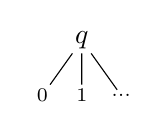
\begin{tikzpicture}[baseline=(root.base),level distance=7mm,inner ysep=0.5mm,sibling distance=5mm]
 \node (root) {$q$}
    child {node {$\scriptstyle 0$}}
    child {node {$\scriptstyle 1$}}
    child {node {$\scriptstyle \ldots$}}
;
\end{tikzpicture}$
\hspace{2cm}
$\sem{\nat \rightarrow \nat} = 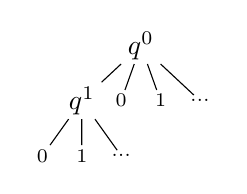
\begin{tikzpicture}[baseline=(root.base),level distance=7mm,inner ysep=0.5mm,sibling distance=5mm]
 \node (root) {$q^0$}
    child{
      node{$q^1$}
      child{node {$\scriptstyle 0$} }
      child{node {$\scriptstyle 1$} }
      child {node {$\scriptstyle \ldots$}}
    }
    child {node {$\scriptstyle 0$}}
    child {node {$\scriptstyle 1$}}
    child {node {$\scriptstyle \ldots$}}
;
\end{tikzpicture}$
\item \highlight{Play} = sequence of moves played alternatively by O and P with justification pointers.
\item \highlight{Strategy for P} = prefix-closed set of plays. $s  a  b$ in the strategy means that
P should respond $b$ when O plays $a$ in position $s$.
\item The \highlight{denotation} of a term $M$, written $\sem{M}$, is a strategy for P.
\item $\sem{ 7 : \nat} = \{ \epsilon, q, q\ 7 \}$\\
$\sem{ \pcfsucc : \nat \rightarrow \nat} = Pref( \{ q^0 q^1 n ( n+1)
\ | \ n \in \nat \} )$
\item Compositionality: $\sem{ \pcfsucc\  7} = \sem{ \pcfsucc } ; \sem{7}$
\end{itemize}
}

\def\highlightat#1#2{\temporal<#1>{#2}{\underline{#2}}{\textcolor{blue}{#2}}}

\section{Computation trees and traversals}
\frame{ \frametitle{Computation trees and traversals}
\highlight{\it Computation tree:} AST of the $\eta$-long normal form of a term.

Example: $M \equiv \lambda f z .
(\lambda g x . f x) (\lambda y. y) z$ of type $(o \typear o) \typear
o \typear o$. \vspace{0.5cm}
\begin{columns}
\column{6cm}
 \visible<2->{\highlight{\it Traversal:} justified
sequence of nodes representing the computation. }

\setbox0=\hbox{$\textcolor{blue}{
\pstr{\only<3->{\nd t= (q1){\lambda f z}}
        \only<4->{\nd \cdot (n2-q1) {@}}
        \only<5->{\nd \cdot (n3-n2){\lambda g x}}
        \only<6->{\nd \cdot (q3-q1,35){f}}
        \only<7->{\nd \cdot (q4-q3){\lambda}}
        \only<8->{\nd \cdot (n8-n3,35){x}}
        \only<9->{\nd \cdot (n9-n2,30){\lambda}}
        \only<10->{\nd \cdot (q2-q1,30){z}}
}}$}
\ht0 1cm\box0 % Make sure the height of box containing the traversal remains constant across the different generated slides

\vspace*{0.5cm}
\visible<11->{\highlight{\it Traversal reduction:} keep only
nodes hereditarily justified by the root.
$\color{red}{
\Pstr[0.7cm]{t \upharpoonright r = (q1){\lambda f z} \cdot (q3-q1,50){f}
\cdot (q4-q3,50){\lambda} \cdot (q2-q1){z} } }$
}

\vspace*{0.8cm}
\visible<12->{
\highlight{\it @-nodes removal:}
 $\Pstr[0.7cm]{ t - @ = (q1){\lambda f z}
 \cdot (n3-q1){ \lambda g x}
 \cdot (q3-q1,35){ f}
 \cdot (q4-q3){ \lambda}
 \cdot (n8-n3,30){ x}
 \cdot (n9-q1,30){ \lambda}
 \cdot (q2-q1,35){z}
} $}
\column{3.5cm}
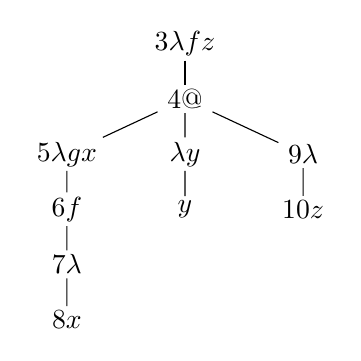
\begin{tikzpicture}[level distance=7mm,inner ysep=0.5mm]
 \node {\highlightat{3}{$\lambda f z$}}
    child {
        node {\highlightat{4}{@}}
        child {
            node {\highlightat{5}{$\lambda g x$}}
            child{
                node{\highlightat{6}{$f$}}
                child {
                    node{\highlightat{7}{$\lambda$}}
                    child {
                        node{\highlightat{8}{$x$}}
                    }
                }
            }
        }
        child {
            node {$\lambda y$}
            child{ node {$y$} }
        }
        child {
            node {$\highlightat{9}{\lambda}$}
            child{ node {\highlightat{10}{$z$}} }
            }
        };
\end{tikzpicture}
\end{columns}
}

%%%%%%%%%%%%%%%%%%%%%%%%%%%%%%%%%%%%%%%%%%%%%%%%%

\section{The Correspondence Theorem}
\frame{ \frametitle{The Correspondence Theorem}
\begin{block}{}
Let $M$ be a simply typed term of type $T$. There exists a partial function $\textcolor{DarkGreen}{\varphi}$
from the nodes of the \highlight{computation tree} to the
moves of the \highlight{arena} $\sem{T}$ such that
$$ \textcolor{DarkGreen}{\varphi}  : \travset(M)^{-@} \textcolor{DarkGreen}{\stackrel{\cong}{\longrightarrow}} \intersem{M} $$
$$ \textcolor{DarkGreen}{\varphi}  : \travset(M)^{\upharpoonright r}  \textcolor{DarkGreen}{\stackrel{\cong}{\longrightarrow}} \sem{M} \ .$$
\end{block}
where
\begin{itemize}
\item $\highlight{\travset(M)}$ = set of traversals of the computation tree of $M$
\item $\highlight{\travset(M)^{\upharpoonright r}} = \{ t \upharpoonright r \ | \  t \in {\travset(M)} \}$
\item $\highlight{\travset(M)^{-@}} = \{ t - @ \ | \  t \in {\travset(M)} \}$
\item $\highlight{\sem{M}}$ = game-semantic denotation of $M$
\item $\highlight{\intersem{M}}$ = revealed denotion ({\it i.e.}~internal moves are uncovered.)
\end{itemize}

}

%%%%%%%%%%%%%%%%%%%%%%%%%%%%%%%%%%%%%%%%%%%%%%%%%
\section{The Correspondence Theorem (example)}
\frame{\frametitle{The Correspondence Theorem (example)}
\begin{center}
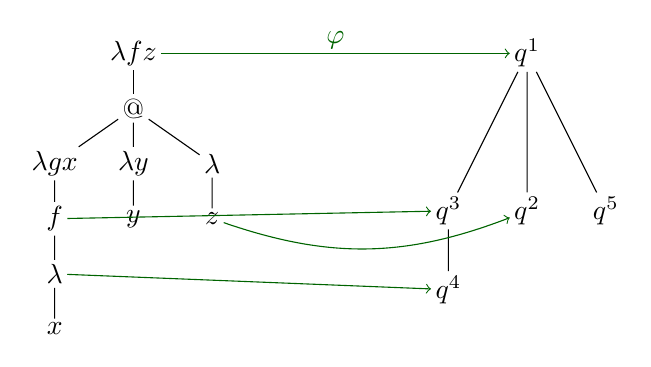
\begin{tikzpicture}[level distance=7mm,inner ysep=0.5mm,inner xsep=0.5mm,sibling distance=10mm]
%\color{blue}
\node (root) {$\lambda f z$}
    child{
      node{$@$}
          child{
            node {$\lambda g x$}
            child{
              node (f) {$f$}
              child{
                node (lmd) {$\lambda$}
                child{
                  node {$x$}
                }
              }
            }
          }
          child{
            node {$\lambda y$}
            child{
              node {$y$}
            }
          }
          child{
            node {$\lambda$}
            child{
              node (z) {$z$}
            }
          }
      }
;
%\color{red}
\draw +(5,0) node (q1) {$q^1$}
    [level distance=20mm]
      child{
        node (q3) {$q^3$}
        [level distance=10mm]
        child{ node (q4) {$q^4$} }
      }
      child{ node (q2) {$q^2$} }
      child{ node (q5) {$q^5$} }
;
\color{DarkGreen}
\draw[->] (root) -- node[above] {$\varphi$} (q1);
\draw[->] (f) -- (q3);
\draw[->] (lmd) -- (q4);
\draw[->] (z) to [bend right=20]  (q2);
\end{tikzpicture}
\end{center}
Take the traversal
%\textcolor{blue}
{\Pstr{t = (q1){\lambda f z} \cdot (n2){@}
\cdot (n3-n2){\lambda g x}
\cdot (q3-q1,35){f}
\cdot (q4-q3){\lambda}
\cdot (n8-n3){x}
\cdot (n9-n2,35){\lambda}
\cdot (q2-q1,35){z}}}. We have:
$
\textcolor{DarkGreen}{
\varphi (} %\textcolor{blue}
{t \upharpoonright r}
\textcolor{DarkGreen}{)} = \textcolor{DarkGreen}{\varphi (}
\textcolor{blue}{
\Pstr[70mm]{ (q1){\lambda f z}
            \cdot (q3-q1){f}
            \cdot (q4-q3){\lambda}
            \cdot (q2-q1){z} }
}
\textcolor{DarkGreen}{)} = %\textcolor{red}
{
\Pstr[70mm]{
    (q1){q}^1\
    (q3-q1){q}^3\
    (q4-q3){q}^4\
    (q2-q1){q}^2
}}
\in %\textcolor{red}
{\sem{M}}.
$
}

%%%%%%%%%%%%%%%%%%%%%%%%%%%%%%%%%%%%%%%%%%%%%%%%%

\section{The Correspondence Theorem (2)}
\frame{ \frametitle{The Correspondence Theorem (2)}
\begin{center}
\begin{tabular}{c|c}
Computation tree notion & Game-semantic equivalent \\ \hline \hline \\
computation tree & arena \\ \\
traversals & uncovered plays \\ \\
reduced traversal & plays \\ \\
paths in the computation tree & P-views of uncovered plays
\end{tabular}
\end{center}
}


%%%%%%%%%%%%%%%%%%%%%%%%%%%%%%%%%%%%%%%%%%%%%%%%%

\section{Game-semantic Characterisation of Safety}
\frame{ \frametitle{Game-semantic Characterisation of Safety}

\begin{itemize}
\item The computation tree of  a safe term is \highlight{incrementally-bound} :
each variable $x$ is bound by the first $\lambda$-node occurring in
\textcolor{red}{the path to the root} with order $> \ord{x}$.
\pause

\item Using the Correspondence Theorem, since paths in the computation tree correspond to P-views
of plays in game semantic, we can show:

\begin{block}{Proposition}
Safe terms are denoted by \highlight{P-incrementally justified strategies}: each P-move $m$ points to the
last O-move in \textcolor{red}{the P-view} with order $> \ord{m}$.
\end{block}
\end{itemize}
\pause

\begin{block}{Corollary}
Justification pointers attached to P-moves are redundant in the game-semantics of safe
terms.
\end{block}
}




%%%%%%%%%%%%%%%%%%%%%%%%%%%%%%%%%%%%%%%%%%%%%%%%%
\section{Conclusion and Future Works}
\frame{ \frametitle{Conclusion and Future Works}

\highlight{Conclusion:}

Safety is a syntactic constraint with interesting algorithmic and
game-semantic properties.

\highlight{Future works:}
\begin{itemize}
\item Find a categorical model of Safe PCF.
\item Complexity classes characterised with the Safe $\lambda$-calculus?
\item Safe Idealized Algol: is contextual equivalence decidable
for some finitary fragment (e.g.~Safe IA$_4$)?
\end{itemize}


\highlight{Related works:}
\begin{itemize}
\item Jolie G. de Miranda's thesis on unsafe grammars.
\item Ong introduced computation trees in LICS2006 to prove decidability of MSO theory on infinite trees
generated by higher-order grammars (whether safe or not).
%\item Stirling recently proved decidability of higher-order pattern matching with a game-semantic approach
%relying on equivalent notions of computation tree and traversal.
\end{itemize}
}


%%%%%%%%%%%%%%%%%%%%%%%%%%%%%%%%%%%%%%%%%%%%%%%%%
\section{Bibliography}

\end{document}
\endinput

\begin{frame} \frametitle<presentation>{Bibliography}

%  \begin{thebibliography}{10}
  \beamertemplatearticlebibitems
    \bibitem{abramsky:game-semantics-tutorial}
    Samson Abramsky and Guy McCusker.
    \newblock Game semantics, Lecture notes.
    \newblock In {\em Proceedings of the 1997 Marktoberdorf Summer School}. Springer-Verlag, 1998.

    \bibitem{safety-mirlong2004}
    Klaus Aehlig, Jolie~G. de~Miranda, and C.-H.~Luke Ong.
    \newblock Safety is not a restriction at level 2 for string languages.
    \newblock Technical report. University of Oxford, 2004.

    \bibitem{OngLics2006}
    C.-H.~Luke Ong.
    \newblock On model-checking trees generated by higher-order recursion schemes.
    \newblock In {\em Proceedings of LICS.} Computer Society Press, 2006.

%    \bibitem{DBLP:conf/icalp/Stirling06}
%    Colin Stirling
%    \newblock A Game-Theoretic Approach to Deciding Higher-Order Matching.
%    \newblock In {\em Proceedings of ICALP.} Springer, 2006.

%  \end{thebibliography}
\end{frame}

\end{document}


\pstrSetArrowColor{black}

\title{\texorpdfstring{The Safe $\lambda$-Calculus}{The Safe Lambda-Calculus}}

\author[W. Blum, C.-H. L. Ong]{\texorpdfstring{\\ William Blum\\ \ \\
 Joint work with C.-H. Luke Ong}{William Blum}}


\institute[University Of Oxford]{Oxford University Computing Laboratory}

\date{\small \color{red}{Lunch-time meeting, 14 May 2007}}


\begin{document}

\section{Title page}
  \frame{\titlepage}


%\section<presentation>*{Outline}
%\begin{frame}
%  \frametitle{Outline}
%  \tableofcontents[part=1]
%\end{frame}
%\AtBeginSection[] {
%   \begin{frame}<beamer>
%     \frametitle{Outline}
%     \tableofcontents[currentpart,currentsection]
%   \end{frame}
% }
%
%\part<presentation>{Main Talk}

%%%%%%%%%%%%%%%%%%%%%%%%%%%%%%%%%%%%%%%%%%%%%%%%%

\section{Overview}
\frame{\frametitle{Overview}

\begin{itemize}
\item \highlight{Safety} is originally a syntactic restriction for higher-order grammars
with nice automata-theoretic characterization.
\item In the context of the $\lambda$-calculus it gives rise to the \highlight{Safe $\lambda$-calculus}.
\item The loss of expressivity can be characterized in terms of representable numeric functions.
\item The calculus has a ``succinct'' game-semantic model.
\end{itemize}
}


%%%%%%%%%%%%%%%%%%%%%%%%%%%%%%%%%%%%%%%%%%%%%%%%%

\section{Outline for this talk}
\frame{
\frametitle{Outline for this talk}
\begin{description}
\item[Part I] The safety restriction
\begin{enumerate}
\item Safety for higher-order grammars
\item The safe $\lambda$-calculus
\item Expressivity
\end{enumerate}
\item[Part II] Game-semantic
\begin{enumerate}
\item The Correspondence Theorem
\item Game-semantic characterisation
\item Compositionality
\end{enumerate}
\end{description}
}


\part{The Safety Restriction}
\frame{
\begin{center}
\bf \Huge Part I :
The Safety Restriction
\end{center}
}


\section{Higher-order grammars}
\frame{\frametitle{Higher-order grammars}
\emph{Notation for types:} $A_1 \rightarrow (A_2 \rightarrow (\ldots (A_n \rightarrow o)) \ldots )$
is written $(A_1,A_2,\ldots, A_n,o)$.

\begin{itemize}

\item Higher-order grammars (Maslov, 1974) are used as generators of word languages, trees or graphs.

\item A \highlight{higher-grammar} is formally given by a tuple
$\langle \Sigma, \mathcal{N}, \mathcal{R}, \mathcal{S} \rangle$
(terminals, non-terminals, rewritting rules, starting symbol)

\item Example of a tree-generating order-2 grammar:
\begin{columns}
      \column{.3\textwidth}
$\begin{array}{rll}
  S & \rightarrow & H \, a\\
  H \, z^o & \rightarrow & F \, (g \,
  z)\\
  F \, \phi^{(o, o)} & \rightarrow & \phi \, (\phi \, (F \, h))\\
\end{array}$
      \column{.3\textwidth}
\begin{tikzpicture}[baseline=(root.base),level distance=5mm,inner ysep=0.5mm,sibling distance=10mm]
 \node (root) {$g$}
    child {node {$a$}}
    child {node {$g$}
        child { node{$a$} }
        child { node{$h$}
                child { node{$h$}
                        child { node{$\vdots$} }
                }
        }
    } ;
\end{tikzpicture}
\end{columns}
Non-terminals: $S :o$, $H:(o,o)$ and $F:((o,o),o)$. Terminals: $a:o$ and $g,h:(o,o)$.
\end{itemize}
}

%%%%%%%%%%%%%%%%%%%%%%%%%%%%%%%%%%%%%%%%%%%%%%%%%
\section{The Safety Restriction}
\frame{\frametitle{The Safety Restriction}
\begin{itemize}
\item First appeared under the name ``restriction of derived types'' in ``IO and OI Hierarchies'' by W. Damm, TCS 1982
\item It is a \highlight{syntactic restriction} for higher-order grammars that constrains the occurrences
of the variables in the grammar equations according to their orders.
\pause

\item $(A_1, \cdots, A_n, o)$ is \highlight{homogeneous} if
$A_1$, \ldots, $A_n$ are and $\ord{A_1} \geq \ord{A_2}\geq \cdots \geq \ord{A_n}$.
\end{itemize}

\begin{definition}[Knapik, Niwi\'nski and Urzyczyn (2001-2002)]
\noindent All types are assumed to be \emph{homogeneous}.

  An order $k > 0$ term is \emph{unsafe} if it contains an
  occurrence of a parameter of order strictly less than $k$.
  An unsafe subterm $t$ of $t'$ occurs in \emph{safe position}
  if it is in operator position ($t' = \cdots (ts) \cdots$).
  A grammar is \highlight{safe} if at the right-hand side of any production
  all unsafe subterms occur in safe positions.
\end{definition}
}

\section{Some Results On Safety}
\frame{\frametitle{Some Results On Safety}
\begin{description}
\item [Damm82] For generating word languages, order-$n$ safe grammars are
equivalent to order-$n$ pushdown automata.

\item [KNU02] Generalization of Damm's result to
\emph{tree generating} safe grammars/PDAs.

\item [KNU02] The Monadic Second Order (MSO) model checking problem for trees generated by
    \highlight{safe} higher-order grammars of any order is decidable.

\item [Ong06] But anyway, KNU02 result's is also true for unsafe grammars...

\item [Caucal02] Graphs generated by safe grammars have a decidable MSO theory.

\item [HMOS06] Caucal's result does not extend to unsafe grammars.
However deciding $\mu$-calculus theories is $n$-EXPTIME complete.

\item [AdMO04] Proposed a notion of safety for the $\lambda$-calculus (unpublished).

\end{description}


\note{
\begin{itemize}
\item nPDA = finite state machines + order n stack
\item For words: 1PDA recognizes context-free language.
        and 0PDA = recognizes regular language.
\item MSO is very expressive: more than the modal mu-calculus (into which LTL CTL CTL* can be embedded.
But over trees, MSO and modal mu-calculus are equi-expressive.)
\end{itemize}
}
}



%%%%%%%%%%%%%%%%%%%%%%%%%%%%%%%%%%%%%%%%%%%%%%%%%
\section{Simply Typed \texorpdfstring{$\lambda$}{Lambda}-Calculus}
\frame{\frametitle{Simply Typed $\lambda$-Calculus}
\begin{itemize}
\item \highlight{Simple types} $A := o\ |\ A \rightarrow A$.
%We write $(A_1,\ldots, A_n)$ for $A_1\rightarrow \ldots \rightarrow A_n$.

\item The \highlight{order} of a type is given by $\textsf{order}(o) = 0$,
$\textsf{order}(A \rightarrow B) = \max(\textsf{order}(A) + 1, \textsf{order}(B))$.

\item Jugdements of the form $ \Gamma \vdash M : T $ where $\Gamma$ is the context, $M$ is the term and $T$ is the type:
$$ \rulename{var} \   \rulef{}{x : A\vdash x : A}
\qquad  \rulename{wk} \   \rulef{\Gamma \vdash M : A}{\Delta \vdash M : A} \ \Gamma \subset \Delta$$
$$ \rulename{app} \  \rulef{\Gamma \vdash M : A \rightarrow B \quad \Gamma \vdash N : A }
                           {\Gamma  \vdash M N : B}
\quad \rulename{abs} \   \rulef{\Gamma, x : A \vdash M : B}
                                {\Gamma  \vdash \lambda x^A. M : A \rightarrow B}$$

\item Example: $f:o\rightarrow o\rightarrow o, x:o \vdash (\lambda \varphi^{o \rightarrow o} x^o . \varphi\ x) (f\ x)$

\item A single rule: \highlight{$\beta$-reduction}. e.g. $(\lambda x. M) N \betared M [N/x]$
\end{itemize}
}




%%%%%%%%%%%%%%%%%%%%%%%%%%%%%%%%%%%%%%%%%%%%%%%%%
\section{The Safe \texorpdfstring{$\lambda$}{Lambda}-Calculus}
\begin{frame} \frametitle{The Safe $\lambda$-Calculus}

\begin{block}{The formation rules}
$$ \rulename{var} \   \rulef{}{x : A\vdash_s x : A}
\qquad  \rulename{wk} \   \rulef{\Gamma \vdash_s M : A}{\Delta \vdash_s
M : A} \ \Gamma \subset \Delta$$
$$ \rulename{app} \  \rulef{\Gamma \vdash M : (A_1,\ldots,A_l,B)
                                        \quad \Gamma \vdash_s N_1 : A_1
                                        \quad \ldots \quad \Gamma \vdash_s N_l : A_l  }
                                   {\Gamma  \vdash_s M N_1 \ldots N_l : B}$$
\hfill with the side-condition $\textcolor{red}{\forall y \in \Gamma
: \ord{y} \geq \ord{B}}$
$$ \rulename{abs} \   \rulef{\Gamma, x_1:A_1 \ldots x_n : A_n \vdash_s M : B}
                                   {\Gamma  \vdash_s \lambda x_1:A_1 \ldots x_n : A_n . M : A_1 \rightarrow \ldots \rightarrow A_n \rightarrow B}$$
\hfill with the side-condition $\textcolor{red}{\forall y \in \Gamma
: \ord{y} \geq \ord{A_1 \rightarrow \ldots \rightarrow A_n
\rightarrow B}}$
\end{block}

\begin{lemma}
  If $\Gamma \vdash_s M : A$ then every free variable in $M$ has order at least $\ord{A}$.
\end{lemma}

\end{frame}

%%%%%%%%%%%%%%%%%%%%%%%%%%%%%%%%%%%%%%%%%%%%%%%%%

\section{Variable Capture}
\frame{\frametitle{Variable Capture} \highlight{The usual
``problem'' in $\lambda$-calculus}: avoid \alert{variable capture}
when performing substitution: $ (\lambda x . (\lambda y . x)) y
\betared (\lambda \underline{y} . x) [\underline{y}/x] \neq \lambda
y . y$\pause
\begin{enumerate}
\item \highlight{Standard solution}: Barendregt's convention. Variables are renamed so that free variables and bound variables have different names.
Eg. $(\lambda x . (\lambda y . x)) y$ becomes $(\lambda x . (\lambda
z . x)) y$ which reduces to $(\lambda z . x) [y/x] = \lambda z . y$
\pause

\alert{Drawback:} requires to have access to an unbounded supply of names to perform
a given sequence of $\beta$-reductions.
\note{Drawback 1, eg. $(\lambda x_1 \ldots x_n . (\lambda y_1 \ldots y_n . x_1 \ldots x_n)) y_1 \ldots y_n$}
\pause

\item \highlight{Another solution}: use the $\lambda$-calculus \`a la de Brujin where variable binding is specified by an index instead of a name.
Variable renaming then becomes unnecessary.
\pause

\alert{Drawback:} the conversion to nameless de Brujin $\lambda$-terms requires an unbounded supply of indices.
\end{enumerate}

\pause
\begin{block}{Property}
In the Safe $\lambda$-calculus there is no need to rename variables when
performing substitution.
\end{block}

}

%%%%%%%%%%%%%%%%%%%%%%%%%%%%%%%%%%%%%%%%%%%%%%%%%
\section{Examples}
\frame{\frametitle{Examples}
\begin{enumerate}
\item
Contracting the $\beta$-redex in the following term
$$f:o\rightarrow o\rightarrow o, x:o \vdash (\lambda \varphi^{o \rightarrow o} x^o . \varphi\ x) (\temporal<2>{f\ x}{\underline{f\ \alert{x}}}{\underline{f\ \alert{x}}})$$
leads to variable capture:
$$(\lambda \varphi x . \varphi\ x) (f\ x) \not\betared (\lambda \alert{x} . (f\ \alert{x}) x).$$
\pause
Hence the term is \alert{unsafe}. Indeed, $\ord{x} = 0 \leq 1 = \ord{f\ x}$.
\pause

\item The term $(\lambda \varphi^{o \rightarrow o} x^o . \varphi\ x) (\lambda y^o . y )$ is safe.
\pause

\item Safety does not capture ``variable-renaming uselessness''. E.g.~the unsafe term
$\lambda y^o z^o. (\lambda x^o .y) z$ can be contracted using capture-permitting substitution.
\pause

\item Up to order $2$, $\beta$-normal terms are always safe.
\pause

\item \highlight{Kierstead terms} $\lambda f^{((o,o),o)} . f (\lambda x^o . f (\lambda y^o . y
))$ is safe but $\lambda f^{((o,o),o)} . f (\lambda x^o . f (\underline{\lambda y^o .x}))$ is unsafe.

\end{enumerate}
}

%%%%%%%%%%%%%%%%%%%%%%%%%%%%%%%%%%%%%%%%%%%%%%%%%
\section{Transformations preserving safety}
\frame{\frametitle{Transformations preserving safety}
\begin{itemize}
  \item Substitution preserves safety.
  \pause
  \item $\beta$-reduction does not preserve safety:
Take  $w,x,y,z : o$ and $f : (o,o,o)$.
The safe term $(\lambda x y . f\ x\ y) z\ w$
$\beta$-reduces to the unsafe term $(\underline{\lambda y . f\ z\ y}) w$
which in turns reduces to the safe term $f\ z\ w$.
  \pause

  \item Safe $\beta$-reduction: reduces simultaneously as many $\beta$-redexes
as needed in order to reach a safe term.
  \item Safe $\beta$-reduction preserves safety.
  \pause
  \item $\eta$-reduction preserves safety.
  \pause
  \item $\eta$-expansion \alert{does not} preserve safety. E.g.~
  $\vdash_s \lambda y^o z^o . y : (o,o,o)$ but
$\not \vdash_s \lambda x^o . (\lambda y^o z^o . y) x : (o,o,o)$.
  \pause
  \item $\eta$-long normal expansion preserves safety.
\end{itemize}

}


\section{Expressivity}
\frame{ \frametitle{Expressivity}

Safety is a strong constraint but it
is still unclear how it restricts expressivity:
\begin{itemize}
\item de Miranda showed that at order 2 for word languages,
non-determinism palliates the loss of expressivity.
It is unknown if this extends to higher orders.

\item For tree-generating grammars: Urzyczyn conjectured that
safety is a proper constraint i.e.~that there is a tree which is intrinsically unsafe.
He proposed a possible counter-example.

\item For graphs, HMOS06's undecidability result implies that safety restricts expressivity.

\item For simply-typed terms: ...

\end{itemize}
}

%%%%%%%%%%%%%%%%%%%%%%%%%%%%%%%%%%%%%%%%%%%%%%%%%
\section{Numerical functions}
\frame{ \frametitle{Numerical functions}

Church Encoding: for $n\in\nat$, $\overline{n} = \lambda s z. s^n z$
of type $I = (o\rightarrow o)\rightarrow o\rightarrow o$.

\begin{theorem}[Schwichtenberg 1976]
The numeric functions representable by simply-typed terms of type $I\rightarrow \ldots \rightarrow I$ are
exactly the multivariate polynomials extended with the conditional function:
$$ cond(t,x,y) =
\left\{ \begin{array}{ll} x, & \mbox{if $t=0$} \\
y, & \mbox{if $t = n+1$}\ .
\end{array} \right.
$$
\end{theorem}
$cond$ is represented by the term $C = \lambda F G H \alpha x . H (
\temporal<2>{\lambda y . G \alpha x}
{\underline{\lambda y . G \alpha x}}{\underline{\lambda y . G \alpha x}}
 ) (F \alpha x)$.
\pause
\begin{theorem}
Functions representable  by safe $\lambda$-expressions of type $I\rightarrow \ldots \rightarrow I$  are
exactly the multivariate polynomials.
\end{theorem}
So $cond$ is not representable in the Safe $\lambda$-calculus and $C$ is unsafe.
}

%%%%%%%%%%%%%%%%%%%%%%%%%%%%%%%%%%%%%%%%%%%%%%%%%

%%%%\section{Game Semantics}
%%%%\frame{ \frametitle{Game Semantics}
%%%%Let $\vdash M:T$ be a pure simply typed term.
%%%%
%%%%\begin{itemize}
%%%%\item \highlight{Game-semantics} provides a model of $\lambda$-calculus.
%%%%$M$ is denoted by a strategy $\sem{M}$ on a 2-player game induced by $T$.
%%%%\item A \highlight{strategy} is represented by a set of sequences of moves together with \highlight{links}: each move points
%%%%to a preceding move.
%%%%\pause
%%%%\item \textcolor{DarkGreen}{Computation tree} = canonical tree representation of a term.
%%%%\item \textcolor{DarkGreen}{Traversals $\travset(M)$ } = sequences of nodes with links respecting some formation rules.
%%%%\end{itemize}
%%%%\pause
%%%%
%%%%\begin{block}{The Correspondence Theorem}
%%%%The game semantics of a term can be represented on the computation
%%%%tree:
%%%%$$ \textcolor{DarkGreen}{\travset(M)} \cong \textcolor{blue}{\intersem{M}} $$
%%%%$$ \textcolor{DarkGreen}{Reduction(\travset(M))} \cong \textcolor{blue}{\sem{M}}$$
%%%%where $\textcolor{blue}{\intersem{M}}$ is the revealed game-semantic denotion (i.e. internal moves are uncovered).
%%%%\end{block}
%%%%}


%%%%%%%%%%%%%%%%%%%%%%%%%%%%%%%%%%%%%%%%%%%%%%%%%

\part{Game semantics}
\frame{
\begin{center}
\bf \Huge Part II :
Game semantics
\end{center}
}

\section{Game semantics}
\frame{\frametitle{Game semantics}
 Model of programming languages based on games (Abramsky et al.; Hyland and Ong; Nickau)
\begin{itemize}
\item 2 players: \highlight{O}pponnent (system) and \highlight{P}roponent (program)
\item The term type induces an \highlight{arena} defining the possible moves
$\sem{\nat} = 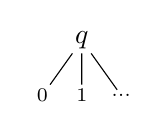
\begin{tikzpicture}[baseline=(root.base),level distance=7mm,inner ysep=0.5mm,sibling distance=5mm]
 \node (root) {$q$}
    child {node {$\scriptstyle 0$}}
    child {node {$\scriptstyle 1$}}
    child {node {$\scriptstyle \ldots$}}
;
\end{tikzpicture}$
\hspace{2cm}
$\sem{\nat \rightarrow \nat} = 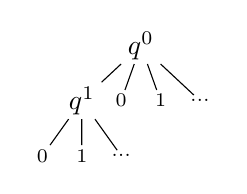
\begin{tikzpicture}[baseline=(root.base),level distance=7mm,inner ysep=0.5mm,sibling distance=5mm]
 \node (root) {$q^0$}
    child{
      node{$q^1$}
      child{node {$\scriptstyle 0$} }
      child{node {$\scriptstyle 1$} }
      child {node {$\scriptstyle \ldots$}}
    }
    child {node {$\scriptstyle 0$}}
    child {node {$\scriptstyle 1$}}
    child {node {$\scriptstyle \ldots$}}
;
\end{tikzpicture}$
\item \highlight{Play} = sequence of moves played alternatively by O and P with justification pointers.
\item \highlight{Strategy for P} = prefix-closed set of plays. $s  a  b$ in the strategy means that
P should respond $b$ when O plays $a$ in position $s$.
\item The \highlight{denotation} of a term $M$, written $\sem{M}$, is a strategy for P.
\item $\sem{ 7 : \nat} = \{ \epsilon, q, q\ 7 \}$\\
$\sem{ \pcfsucc : \nat \rightarrow \nat} = Pref( \{ q^0 q^1 n ( n+1)
\ | \ n \in \nat \} )$
\item Compositionality: $\sem{ \pcfsucc\  7} = \sem{ \pcfsucc } ; \sem{7}$
\end{itemize}
}

\def\highlightat#1#2{\temporal<#1>{#2}{\underline{#2}}{\textcolor{blue}{#2}}}

\section{Computation trees and traversals}
\frame{ \frametitle{Computation trees and traversals}
\highlight{\it Computation tree:} AST of the $\eta$-long normal form of a term.

Example: $M \equiv \lambda f z .
(\lambda g x . f x) (\lambda y. y) z$ of type $(o \typear o) \typear
o \typear o$. \vspace{0.5cm}
\begin{columns}
\column{6cm}
 \visible<2->{\highlight{\it Traversal:} justified
sequence of nodes representing the computation. }

\setbox0=\hbox{$\textcolor{blue}{
\pstr{\only<3->{\nd t= (q1){\lambda f z}}
        \only<4->{\nd \cdot (n2) {@}}
        \only<5->{\nd \cdot (n3-n2){\lambda g x}}
        \only<6->{\nd \cdot (q3-q1,35){f}}
        \only<7->{\nd \cdot (q4-q3){\lambda}}
        \only<8->{\nd \cdot (n8-n3,35){x}}
        \only<9->{\nd \cdot (n9-n2,30){\lambda}}
        \only<10->{\nd \cdot (q2-q1,30){z}}
}}$}
\ht0 1cm\box0 % Make sure the height of box containing the traversal remains constant across the different generated slides

\vspace*{0.5cm}
\visible<11->{\highlight{\it Traversal reduction:} keep only
nodes hereditarily justified by the root.
$\color{red}{
\Pstr[0.7cm]{t \upharpoonright r = (q1){\lambda f z} \cdot (q3-q1,50){f}
\cdot (q4-q3,50){\lambda} \cdot (q2-q1){z} } }$
}

\vspace*{0.8cm}
\visible<12->{
\highlight{\it @-nodes removal:}
 $\Pstr[0.7cm]{ t - @ = (q1){\lambda f z}
 \cdot (n3-q1){ \lambda g x}
 \cdot (q3-q1,35){ f}
 \cdot (q4-q3){ \lambda}
 \cdot (n8-n3,30){ x}
 \cdot (n9-q1,30){ \lambda}
 \cdot (q2-q1,35){z}
} $}
\column{3.5cm}
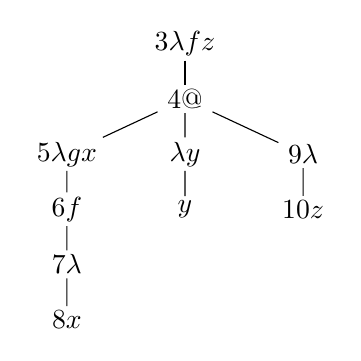
\begin{tikzpicture}[level distance=7mm,inner ysep=0.5mm]
 \node {\highlightat{3}{$\lambda f z$}}
    child {
        node {\highlightat{4}{@}}
        child {
            node {\highlightat{5}{$\lambda g x$}}
            child{
                node{\highlightat{6}{$f$}}
                child {
                    node{\highlightat{7}{$\lambda$}}
                    child {
                        node{\highlightat{8}{$x$}}
                    }
                }
            }
        }
        child {
            node {$\lambda y$}
            child{ node {$y$} }
        }
        child {
            node {$\highlightat{9}{\lambda}$}
            child{ node {\highlightat{10}{$z$}} }
            }
        };
\end{tikzpicture}
\end{columns}
}

%%%%%%%%%%%%%%%%%%%%%%%%%%%%%%%%%%%%%%%%%%%%%%%%%

\section{The Correspondence Theorem}
\frame{ \frametitle{The Correspondence Theorem}
\begin{block}{}
Let $M$ be a simply typed term of type $T$. There exists a partial function $\textcolor{DarkGreen}{\varphi}$
from the nodes of the \highlight{computation tree} to the
moves of the \highlight{arena} $\sem{T}$ such that
$$ \textcolor{DarkGreen}{\varphi}  : \travset(M)^{-@} \textcolor{DarkGreen}{\stackrel{\cong}{\longrightarrow}} \intersem{M} $$
$$ \textcolor{DarkGreen}{\varphi}  : \travset(M)^{\upharpoonright r}  \textcolor{DarkGreen}{\stackrel{\cong}{\longrightarrow}} \sem{M} \ .$$
\end{block}
where
\begin{itemize}
\item $\highlight{\travset(M)}$ = set of traversals of the computation tree of $M$
\item $\highlight{\travset(M)^{\upharpoonright r}} = \{ t \upharpoonright r \ | \  t \in {\travset(M)} \}$
\item $\highlight{\travset(M)^{-@}} = \{ t - @ \ | \  t \in {\travset(M)} \}$
\item $\highlight{\sem{M}}$ = game-semantic denotation of $M$
\item $\highlight{\intersem{M}}$ = revealed denotion ({\it i.e.}~internal moves are uncovered.)
\end{itemize}

}

%%%%%%%%%%%%%%%%%%%%%%%%%%%%%%%%%%%%%%%%%%%%%%%%%
\section{The Correspondence Theorem (example)}
\frame{\frametitle{The Correspondence Theorem (example)}
Left: computation tree. Right: arena.
\begin{center}
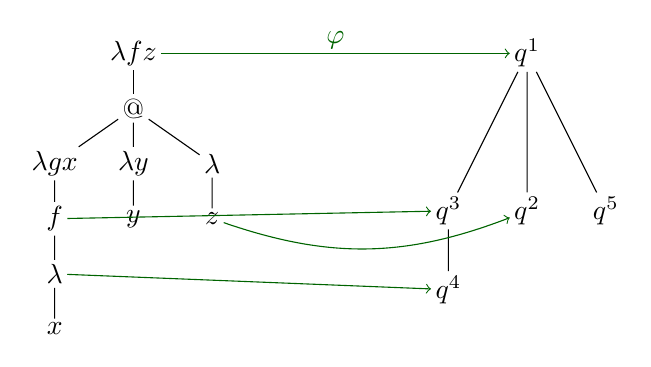
\begin{tikzpicture}[level distance=7mm,inner ysep=0.5mm,inner xsep=0.5mm,sibling distance=10mm]
%\color{blue}
\node (root) {$\lambda f z$}
    child{
      node{$@$}
          child{
            node {$\lambda g x$}
            child{
              node (f) {$f$}
              child{
                node (lmd) {$\lambda$}
                child{
                  node {$x$}
                }
              }
            }
          }
          child{
            node {$\lambda y$}
            child{
              node {$y$}
            }
          }
          child{
            node {$\lambda$}
            child{
              node (z) {$z$}
            }
          }
      }
;
%\color{red}
\draw +(5,0) node (q1) {$q^1$}
    [level distance=20mm]
      child{
        node (q3) {$q^3$}
        [level distance=10mm]
        child{ node (q4) {$q^4$} }
      }
      child{ node (q2) {$q^2$} }
      child{ node (q5) {$q^5$} }
;
\color{DarkGreen}
\draw[->] (root) -- node[above] {$\varphi$} (q1);
\draw[->] (f) -- (q3);
\draw[->] (lmd) -- (q4);
\draw[->] (z) to [bend right=20]  (q2);
\end{tikzpicture}
\end{center}
Take the traversal
%\textcolor{blue}
{\Pstr{t = (q1){\lambda f z} \cdot (n2){@}
\cdot (n3-n2){\lambda g x}
\cdot (q3-q1,35){f}
\cdot (q4-q3){\lambda}
\cdot (n8-n3){x}
\cdot (n9-n2,35){\lambda}
\cdot (q2-q1,35){z}}}. We have:
$
\textcolor{DarkGreen}{
\varphi (} %\textcolor{blue}
{t \upharpoonright r}
\textcolor{DarkGreen}{)} = \textcolor{DarkGreen}{\varphi (}
\textcolor{blue}{
\Pstr[70mm]{ (q1){\lambda f z}
            \cdot (q3-q1){f}
            \cdot (q4-q3){\lambda}
            \cdot (q2-q1){z} }
}
\textcolor{DarkGreen}{)} = %\textcolor{red}
{
\Pstr[70mm]{
    (q1){q}^1\
    (q3-q1){q}^3\
    (q4-q3){q}^4\
    (q2-q1){q}^2
}}
\in %\textcolor{red}
{\sem{M}}.
$
}

%%%%%%%%%%%%%%%%%%%%%%%%%%%%%%%%%%%%%%%%%%%%%%%%%

\section{The Correspondence Theorem (2)}
\frame{ \frametitle{The Correspondence Theorem (2)}
\begin{center}
\begin{tabular}{c|c}
Computation tree notions & Game-semantic equivalents \\ \hline \hline \\
computation tree & arena(s) \\ \\
traversal & uncovered play \\ \\
reduced traversal & play \\ \\
path in the computation tree & P-view of an uncovered play
\end{tabular}
\end{center}
}


%%%%%%%%%%%%%%%%%%%%%%%%%%%%%%%%%%%%%%%%%%%%%%%%%

\section{Game-semantic Characterisation of Safety}
\frame{ \frametitle{Game-semantic Characterisation of Safety}

\begin{itemize}
\item The computation tree of  a safe term is \highlight{incrementally-bound} :
each variable $x$ is bound by the first $\lambda$-node occurring in
\textcolor{red}{the path to the root} with order $> \ord{x}$.
\pause

\item By the Correspondence Theorem, this implies that:
    \begin{block}{Proposition}
    \begin{itemize}
    \item Safe terms are denoted by \highlight{P-incrementally justified strategies}: each P-move $m$ points to the last O-move in \textcolor{red}{the P-view} with order $> \ord{m}$.
    \item Reciprocally, if a \emph{closed} term is denoted by a \highlight{P-incrementally justified strategy} then its $\eta$-long $\beta$-normal form is safe.
    \note{``closed'' is necessary: take $\lambda x y . x$ and $\lambda y . x$.}
    \end{itemize}
    \end{block}
\end{itemize}
\pause

\begin{block}{Corollary}
Justification pointers attached to P-moves are redundant in the game-semantics of safe
terms.
\end{block}
}

\begingroup
\def\sigcol#1{{\color{blue} #1}}
\def\mucol#1{{\color{red} #1}}

\section{Compositionality}
\frame{ \frametitle{Compositionality}

\highlight{Question} Do P-incrementally-justified strategies compose?

\highlight{No.}    Take $\sigcol{\sigma} = \sem{ \vdash_s \lambda x^o v^o .x : o\typear (o,o)}$
 and  $\mucol{\mu} = \sem{ \vdash_s \lambda y^{(o,o)} \varphi^{((o,o),o)}. \varphi (\lambda u^o . y a) : (o,o) \typear (((o,o),o),o)}$ for some constant $a:o$.
We have $\sigcol{\sigma} \fatcompos \mucol{\mu} = \sem{ \lambda x \varphi. \varphi (\underline{\lambda u . x}) }$ which is not P-i.j. by the previous proposition.
\bigskip

$\begin{array}{ccccccccc}
A &  & \multicolumn{2}{c}{B} && \multicolumn{4}{c}{C}\\
\cline{1-1} \cline{3-4} \cline{6-9}
o & \stackrel{\sigcol{\sigma}}\longrightarrow & o, & o & \stackrel{\mucol{\mu}}\longrightarrow & ((o, &o),& o),& o \\ \\
&&&&&&&&\rnode{n0}{\lambda x \varphi \omove  \mucol {\lambda y \varphi}}\\
&&&&&&&\rnode{n1}{\varphi  \pmove \mucol \varphi}\\
&&&&&&\rnode{n2}{\lambda u \omove  \mucol {\lambda u}} \\
&&&  \rnode{n3}{\omove \sigcol {\lambda x v} \pmove \mucol y} \\
\rnode{n4}{x \pmove \sigcol x}
\end{array}
\ncarc[arcangleA=20,arcangleB=20,linecolor=black]{->}{n4}{n0}
\ncarc[arcangleA=30,arcangleB=20,linecolor=red]{->}{n2}{n1}
\ncarc[arcangleA=30,arcangleB=20,linecolor=red]{->}{n1}{n0}
\ncarc[arcangleA=20,arcangleB=20,linecolor=red]{->}{n3}{n0}
\ncarc[arcangleA=20,arcangleB=20,linecolor=blue]{->}{n4}{n3}
$

}
\endgroup


\section{Compositionality 2 }
\frame{ \frametitle{Compositionality 2}
\begin{definition}
A strategy $\sigma : A \rightarrow B$ is \highlight{closed P-incrementally justified} if it P-i.j. and if for every move $m$ initial in $A$ that is contained in some play of $\sigma$ we have $\ord_A m \geq \ord B$.
\end{definition}

    \begin{itemize}
    \item Remark: This property is not preserved up to the Curry isomorphism!
    \item Example: any P-i.j. strategy on $I\rightarrow A$ is closed P-i.j.
    \item Safe terms denotations are closed P-i.j.
    \end{itemize}
\pause
    \begin{block}{Proposition}
    Closed P-incrementally justified strategies compose.
    \end{block}
Hence we have:
\begin{itemize}
\item a category of games and closed P-i.j. strategies,
\item that is not cartesian-closed,
\item which models the safe $\lambda$-calculus.
\end{itemize}
}

\section{Safe PCF}
\frame{ \frametitle{Safe PCF}

\begin{itemize}
\item \highlight{PCF} = $\lambda^{\rightarrow}$ with base type $\nat$ +  successor, predecessor, conditional + Y combinator

\item \highlight{Safe PCF} = Safe fragment of PCF
\end{itemize}

\begin{block}{Proposition}
  Safe PCF terms are denoted by closed P-i.j. strategies.
\end{block}

\begin{block}{Definability}
Let $\sigma$ be a well-bracketed innocent P-i.j. strategy with finite
 view function defined on a PCF arena
 $A_1 \times \ldots \times  A_i \rightarrow B$.
$\sigma$ is the denotation of some term $\overline{x}:\overline{A} \vdash M : B$
such that $\lambda \overline{x} . M$ is safe.
\end{block}
\highlight{Question:} Does this give a fully abstract model with respect to safe contexts?
\alert{Problem:} The quotiented category model is not rational (since
it is not even cartesian closed)!

}

%%%%%%%%%%%%%%%%%%%%%%%%%%%%%%%%%%%%%%%%%%%%%%%%%
\section{Conclusion and Future Works}
\frame{ \frametitle{Conclusion and Future Works}

\highlight{Conclusion:}

Safety is a syntactic constraint with interesting algorithmic and
game-semantic properties.

\highlight{Future works:}
\begin{itemize}
\item Is there a fully abstract model of Safe PCF (with respect to safe contexts)?
\item Complexity classes characterised with the Safe $\lambda$-calculus?
\item Safe Idealized Algol: is contextual equivalence decidable
for some finitary fragment (e.g.~Safe IA$_4$) (with respect to all/safe contexts) ?
\end{itemize}


\highlight{Related works:}
\begin{itemize}
\item Jolie G. de Miranda's thesis on safe/unsafe grammars.
\item Ong introduced computation trees in LICS2006 to prove decidability of MSO theory on infinite trees
generated by higher-order grammars (whether safe or not).
%\item Stirling recently proved decidability of higher-order pattern matching with a game-semantic approach
%relying on equivalent notions of computation tree and traversal.
\end{itemize}
}


%%%%%%%%%%%%%%%%%%%%%%%%%%%%%%%%%%%%%%%%%%%%%%%%%
\section{Bibliography}

\end{document}
\endinput

\begin{frame} \frametitle<presentation>{Bibliography}

%  \begin{thebibliography}{10}
  \beamertemplatearticlebibitems
    \bibitem{abramsky:game-semantics-tutorial}
    Samson Abramsky and Guy McCusker.
    \newblock Game semantics, Lecture notes.
    \newblock In {\em Proceedings of the 1997 Marktoberdorf Summer School}. Springer-Verlag, 1998.

    \bibitem{safety-mirlong2004}
    Klaus Aehlig, Jolie~G. de~Miranda, and C.-H.~Luke Ong.
    \newblock Safety is not a restriction at level 2 for string languages.
    \newblock Technical report. University of Oxford, 2004.

    \bibitem{OngLics2006}
    C.-H.~Luke Ong.
    \newblock On model-checking trees generated by higher-order recursion schemes.
    \newblock In {\em Proceedings of LICS.} Computer Society Press, 2006.

%    \bibitem{DBLP:conf/icalp/Stirling06}
%    Colin Stirling
%    \newblock A Game-Theoretic Approach to Deciding Higher-Order Matching.
%    \newblock In {\em Proceedings of ICALP.} Springer, 2006.

%  \end{thebibliography}
\end{frame}

\end{document}
